% Origen: Secciones/PI - Hardware empleado.md
\chapter{Hardware empleado}
\label{C:hw}

% Figuras de ESTE capítulo + las compartidas. Siempre al principio del archivo.
\graphicspath{{figs/cap2/}{figs/comunes/}}

\begin{destacado}
En este capítulo se describe (1) por qué necesitamos un módulo de aceleración de
hardware en vez de un microcontrolador, (2) qué plataformas de hardware
programable existen, (3) la plataforma empleada, la Red Pitaya STEMlab 125-14, y
la arquitectura de su SoC Zynq-7000, y (4) los periféricos de la placa.
\end{destacado}

%%%%%%%%%%%%%%%%%%%%%%%%%%%%%%%%%%%%%%%%%%%%%%%%%%%%%%%%%%%%%%%%%%%%%%%%%%%%%%%%
\section{Por qué un módulo de aceleración de HW en vez de un microcontrolador}
\label{S:hw-por-que-acelerador}

La respuesta tiene múltiples razones; los dos factores decisivos son la
\textbf{tasa de muestreo} y la \textbf{capacidad de procesamiento}. Partimos del
criterio de diseño: ``el dispositivo debe ser capaz de \textbf{recuperar} pulsos
con flancos del orden de los $\sim 100\,\text{ns}$''. Si deseamos más de 10
muestras en el flanco del pulso (\emph{samples per pulse}, $\text{spp}>10$), hay
que muestrear a $10/100\,\text{ns} = 100$~MSPS o más para resolver su forma.

\begin{table}[H]
\centering
\caption[Tasas de muestreo de los ADC de distintas plataformas]{%
Comparación de las tasas de muestreo de los ADC de distintas
plataformas~\cite{STM32H723,STM32F407}.\label{t:hw-tasas}}
\small
\begin{tabularx}{\textwidth}{|>{\raggedright\arraybackslash}X|c|>{\centering\arraybackslash}p{0.2\textwidth}|>{\centering\arraybackslash}p{0.2\textwidth}|}
\hline
\encabezado \textbf{Tasa de muestreo} & \textbf{Período}
  & \textbf{Muestras en el flanco de 100~ns} & \textbf{Muestras en un pulso de 300~ns} \\ \hline
\textbf{125 MSPS} (Red Pitaya) & 8~ns & \textbf{$\sim$12} & \textbf{$\sim$37} \\ \hline
5 MSPS (ADC de 12 bits del STM32H723/733) & 200~ns & 0,5 & 1,5 \\ \hline
3,6 MSPS (ADC de 16 bits del STM32H7) & 278~ns & 0,36 & $\sim$1 \\ \hline
2,4 MSPS (STM32F407) & 417~ns & 0,24 & 0,72 \\ \hline
\end{tabularx}
\end{table}

Ni siquiera entrelazando los tres ADC del STM32F407 (7,2~MSPS) se llega a una
muestra por flanco. Por eso los analizadores multicanal basados en µC recurren a
un conformado analógico con tiempos del orden de los microsegundos y a
detectores de pico~\cite{Knoll2010}: circuitos analógicos que retienen el valor
pico (o la carga) hasta una operación de descarga. Esto renuncia a medir la forma
del pulso, pero es la solución adecuada si el spp es bajo. Si en cambio
analizamos la \textbf{cantidad de ciclos de reloj disponibles por muestra},
obtenemos lo presentado en la Tabla~\ref{t:hw-plataformas}.

\begin{table}[H]
\centering
\caption[Comparación de plataformas: reloj, ciclos por muestra y ADC]{%
Comparación de plataformas: reloj, ciclos de reloj disponibles por muestra si la
entrada fuera de 125~MSPS, ADC integrado y tasas típicas de
trabajo~\cite{STM32F407,STM32H723,TMS320F2837xD,RedPitayaDocs}.
\label{t:hw-plataformas}}
\footnotesize
\setlength{\tabcolsep}{3pt}
\newcolumntype{Y}{>{\raggedright\arraybackslash}X}
\begin{tabularx}{\textwidth}{|>{\raggedright\arraybackslash}p{0.17\textwidth}|>{\raggedright\arraybackslash}p{0.1\textwidth}|>{\raggedright\arraybackslash}p{0.11\textwidth}|Y|Y|Y|}
\hline
\encabezado \textbf{Plataforma} & \textbf{Tipo} & \textbf{Reloj}
  & \textbf{Ciclos por muestra (a 125~MSPS)} & \textbf{ADC}
  & \textbf{Tasas típicas de trabajo} \\ \hline
\textbf{Cortex-M4F} (STM32F407) & µC & 168~MHz & 1,3
  & integrado: 12 bits, 2,4~MSPS (7,2~MSPS entrelazando 3 ADC)
  & audio de 48--192~kHz; MCA con detector de pico analógico \\ \hline
\textbf{Cortex-M7} (STM32H723/733) & µC & 480~MHz & 3,8
  & integrado: 16 bits a 3,6~MSPS; 12 bits a 5~MSPS
  & MCA digital a 3,6~MSPS con pulsos de µs \\ \hline
\textbf{TI C2000} (F28379D) & µC (DSC) & 200~MHz, 800~MIPS
  & 1,6 por núcleo (6,4 instrucciones sumando 2 núcleos y 2 CLA)
  & integrado: 16 bits a 1,1~MSPS; 12 bits a 3,5~MSPS
  & lazos de control de 10--100~kHz \\ \hline
\textbf{Red Pitaya STEMlab 125-14} & SoC: FPGA + 2~$\times$ Cortex-A9
  & 125~MHz (PL) · 667~MHz (PS)
  & PL: 1, pero en cada ciclo ejecuta todas las etapas a la vez · PS: 5,3 por
    núcleo
  & externo: LTC2145, 14 bits, 125~MSPS
  & \textbf{125~MSPS sostenidos, 2 canales} \\ \hline
\end{tabularx}
\end{table}

Si suponemos que cada canal de muestreo dispone de todo el tiempo de ejecución,
podemos estimar las operaciones que requiere cada muestra; la suma aproximada se
presenta en la Tabla~\ref{t:hw-ops}. Con 4 ciclos por muestra, a un µC sólo le
alcanza para leer el dato y guardarlo en memoria, sin nada del procesamiento que
buscamos en este proyecto. La estimación además es optimista: supone una
operación por ciclo, sin saltos mal predichos ni esperas de memoria. Con los dos
canales son entre 46 y 56 operaciones por par de muestras, es decir, unas
6--7~Gop/s a 125~MSPS.

\begin{table}[H]
\centering
\caption[Operaciones por muestra del procesamiento en un µC]{%
Estimación a primer orden de la cantidad de operaciones por muestra que
requeriría el procesamiento de nuestro proyecto en un µC.\label{t:hw-ops}}
\small
\begin{tabularx}{\textwidth}{|X|c|}
\hline
\encabezado \textbf{Etapa (por muestra, por canal)} & \textbf{Operaciones aprox.} \\ \hline
\textbf{Lectura de la muestra} (cargar desde el \emph{buffer} del DMA y avanzar el
  puntero) & \textbf{2} \\ \hline
Línea de base: acumular, desplazar y restar & 3 \\ \hline
Discriminación con histéresis (umbrales de cruce y de cierre) & 2--3 \\ \hline
Seguimiento del pico (comparar y actualizar, guardar \emph{t\_peak}) & 2--3 \\ \hline
Integrales $Q_\text{total}$ y $Q_\text{cola}$ (con su condición) & 3 \\ \hline
Largo de la ventana y cierre (contador más 2 comparaciones) & 3 \\ \hline
Fuentes de disparo (flancos y niveles) y escudo/veto & 4--6 \\ \hline
Contadores de diagnóstico y marca de tiempo & 2--3 \\ \hline
\textbf{Guardado de la muestra} (escribir en el \emph{buffer} de captura y avanzar el
  índice) & \textbf{2} \\ \hline
\textbf{Total} & \textbf{$\sim$23--28 por muestra} \\ \hline
\end{tabularx}
\end{table}

Acá aparece la ventaja principal de la FPGA: hace \textbf{todas} esas
operaciones \textbf{a la vez}, cada una en su propia etapa del \emph{pipeline}, y por
eso procesa una muestra por ciclo de forma sostenida. Ni siquiera el procesador
de la misma placa (2~$\times$ Cortex-A9 a 667~MHz, unos 10 ciclos por muestra
entre los dos núcleos) puede hacerlo, porque las muestras no le llegan: el bus de
registros entre el PS y la PL atiende una palabra de 32 bits por transacción, sin
ráfagas, y cada transacción tarda 12 ciclos (96~ns) dentro de la PL. Eso da un
techo de $\sim$42~MB/s, contra los 500~MB/s de dos canales a 125~MSPS en
palabras de 16 bits. Otros criterios, igual de importantes, complican el uso de
un µC para este módulo:
\begin{itemize}
  \item \textbf{\emph{Timestamps} y coincidencias multitrigger.} Un µC puede marcar el
    tiempo de un flanco por hardware, con la captura de entrada de un \emph{timer}, sin
    pasar por una interrupción. Lo que no puede es asociar esa marca a la
    muestra del pulso procesado ni resolver coincidencias entre canales en
    tiempo real: eso queda para el software, que depende de la latencia de las
    interrupciones (ISR), variable en decenas o cientos de ns. En la FPGA el
    \emph{timestamp} es el contador de muestras del mismo reloj que el ADC, y las
    coincidencias se resuelven en el mismo ciclo, con tantos canales como se
    instancien.
  \item \textbf{Tiempo muerto determinista.} En la FPGA cada etapa dura un número
    fijo de ciclos, así que el MCA puede declarar un tiempo muerto determinista
    por evento (el largo de la ventana de medición más una cantidad fija de
    ciclos) y contarlo con sus propios contadores. Esto permite \textbf{corregir
    la tasa de conteo}~\cite{Knoll2010}. En un µC el tiempo muerto depende de las
    interrupciones y de la carga del procesador, y con un tiempo muerto variable
    esa corrección pierde validez.
\end{itemize}

%%%%%%%%%%%%%%%%%%%%%%%%%%%%%%%%%%%%%%%%%%%%%%%%%%%%%%%%%%%%%%%%%%%%%%%%%%%%%%%%
\section{Módulos de aceleración de hardware}
\label{S:hw-modulos-aceleracion}

Estos son \textbf{procesadores especializados}~\cite{Crockett2014} que tienen
por lo general los siguientes objetivos:
\begin{itemize}
  \item Liberar al µC de las tareas de cómputo intensivo, tanto en el flujo de
    datos como en el de instrucciones.
  \item Aumentar la capacidad de respuesta (\emph{responsiveness}) del sistema,
    quitándole al procesador esas tareas largas.
  \item Reducir el consumo de potencia.
  \item Tener un mejor manejo de errores a tiempo de ejecución.
\end{itemize}
Se utilizan cuando transferir los datos al acelerador cuesta menos potencia o
tiempo que procesarlos en la CPU.

\begin{figure}[H]
\centering
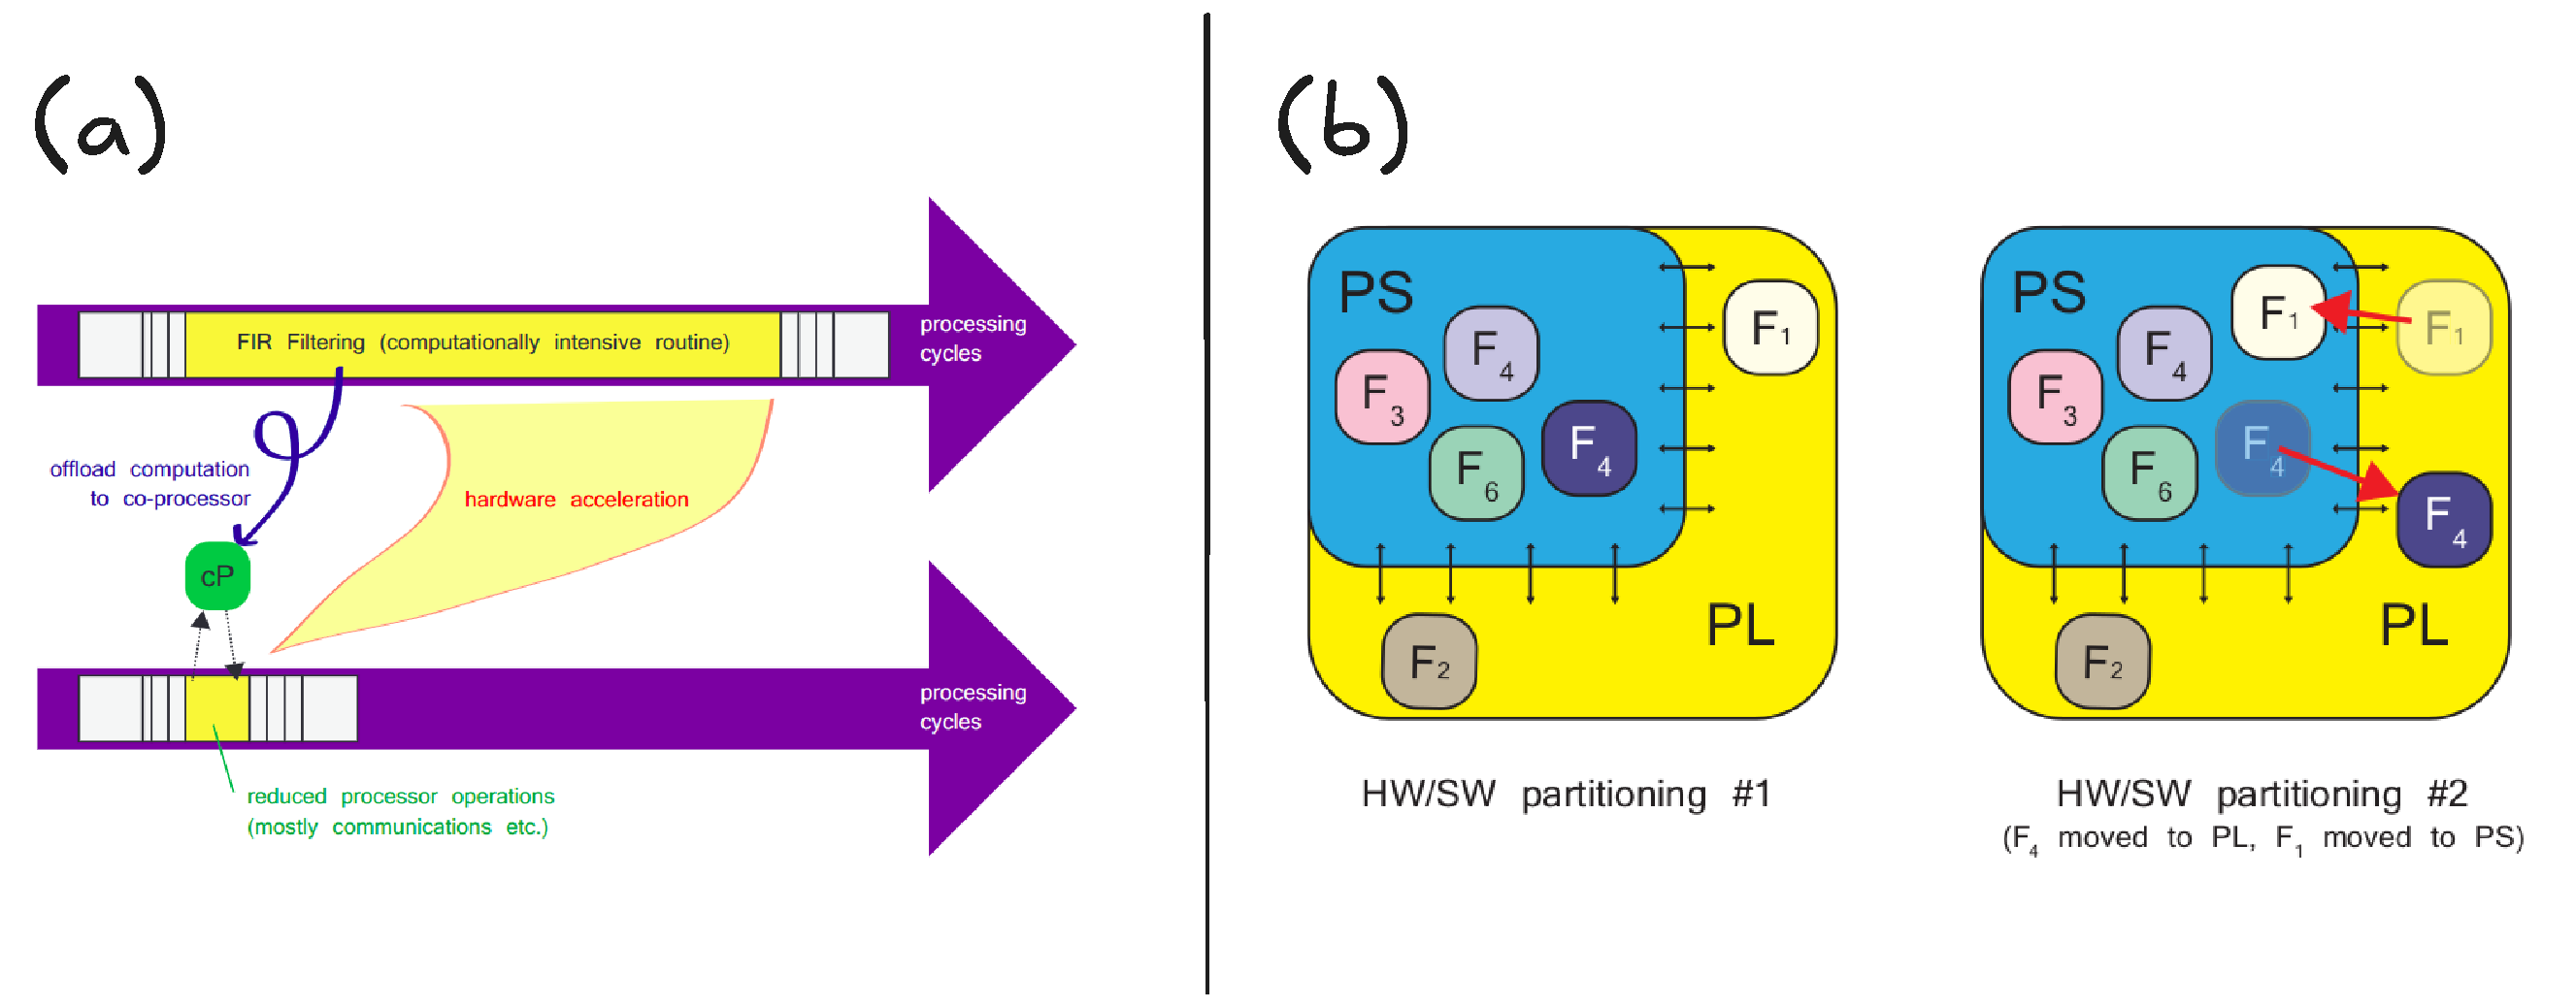
\includegraphics{cap2_offload_uc}
\caption[Aceleradores para reducir la carga de la CPU y particionado HW/SW]{%
Extraídas del ZynqBook~\cite[figs.~4.7 y 4.10]{Crockett2014}. (a)~Utilización
de aceleradores para reducir la carga de la CPU. Arriba, una rutina en la que
una gran parte del tiempo de ejecución está dedicada a una tarea específica, en
este caso un filtrado FIR. Abajo, el filtrado se delega a un coprocesador (cP) y
al procesador le quedan sólo las operaciones de comunicación. (b)~Dos
particionados de tareas HW/SW en un Zynq: en el segundo, F4 pasa a la PL y F1 al
PS.\label{f:hw-offload}}
\end{figure}

Sus usos son diversos, pero generalmente ocupan los siguientes nichos:
\begin{itemize}
  \item \textbf{Computación de baja latencia y determinista}: la respuesta tarda
    un número fijo de ciclos de reloj.
  \item Creación de \textbf{procesadores digitales personalizados de alto
    \emph{throughput}} (DSP).
  \begin{itemize}
    \item Escalabilidad: se pueden crear más canales instanciando más HW, en
      cambio con un µC agregar canales \textbf{quita} ciclos disponibles al
      presupuesto total.
  \end{itemize}
  \item \textbf{Ancho de banda}:
  \begin{itemize}
    \item El \emph{fabric} permite flujos de datos de alto \emph{throughput}. Ejemplo
      con el sistema actual: 125~MSPS $\times$ 14~bits $\approx$
      \textbf{1,75~Gbit/s} sostenidos por canal, 500~MB/s para los dos canales
      en palabras de 16 bits. Un µC no puede procesar ese caudal, y ni siquiera
      guardarlo para después: a ese ritmo, la SRAM del orden de 1~MB de un
      STM32H7 se llena en unos 2~ms.
  \end{itemize}
  \item Interfaz \textbf{directa con el mundo físico} (I/O):
  \begin{itemize}
    \item Necesitamos requisitos de \emph{timing} mucho más ajustados que los que puede
      cumplir una CPU. Incluye:
    \item Interfaz eléctrica del ADC.
  \end{itemize}
  \item \textbf{Descarga de la CPU} (\emph{offload}): la CPU queda libre para
    configurar el hardware, leer los resultados, guardarlos y presentarlos.
  \item Eficiencia energética (ops/W): se eliminan los \emph{fetch}/\emph{decode} de
    instrucciones y los accesos a caché.
  \item \textbf{Flexibilidad en el diseño} (propia de las FPGA): el hardware se
    reconfigura en campo con un \emph{bitstream} nuevo, sin cambiar la placa.
\end{itemize}

%%%%%%%%%%%%%%%%%%%%%%%%%%%%%%%%%%%%%%%%%%%%%%%%%%%%%%%%%%%%%%%%%%%%%%%%%%%%%%%%
\section{Plataformas de HW programable}
\label{S:hw-plataformas-programables}

Las FPGA nacieron en la década de los 80~\cite{Trimberger2015} como herramientas
que permiten la aceleración de hardware personalizada y a costo fijo bajo (entre
los cientos y miles de USD), mientras que los ASIC (\emph{Application Specific
Integrated Circuit}) cuestan entre 3-5 ordenes de magnitud más en su diseño y
producción.

\begin{figure}[H]
\centering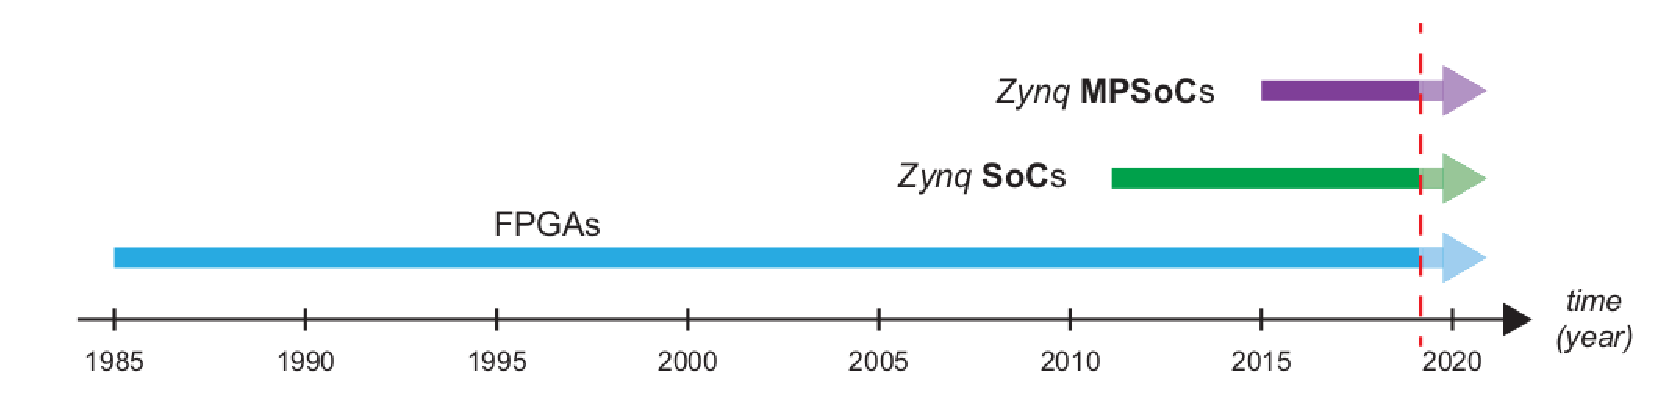
\includegraphics{cap2_historia_plataformas}
\caption[Línea de tiempo de las arquitecturas de HW programable]{%
Linea de tiempo con las principales arquitecturas HW programable.
\label{f:hw-historia}}
\end{figure}

En la Sec.~\ref{S:ap-hw-criterios} se encuentra una tabla exhaustiva de los
criterios de elección de la plataforma de HW~\cite{Crockett2014}; las categorías
principales son recursos computacionales, factores comerciales, facilidad diseño
y desarrollo, características físicas del dispositivo, flexibilidad. En la
Fig.~\ref{f:hw-familias-fpgas}(a) se muestran algunas familias de plataformas y
su aplicabilidad en los ejes capacidad del dispositivo (eje x) vs.\ la dificultad
en el diseño y desarrollo (eje y). En la Fig.~\ref{f:hw-familias-fpgas}(b) se
presenta la evolución de los recursos lógicos configurables, representados en
área.

\begin{figure}[H]
\centering
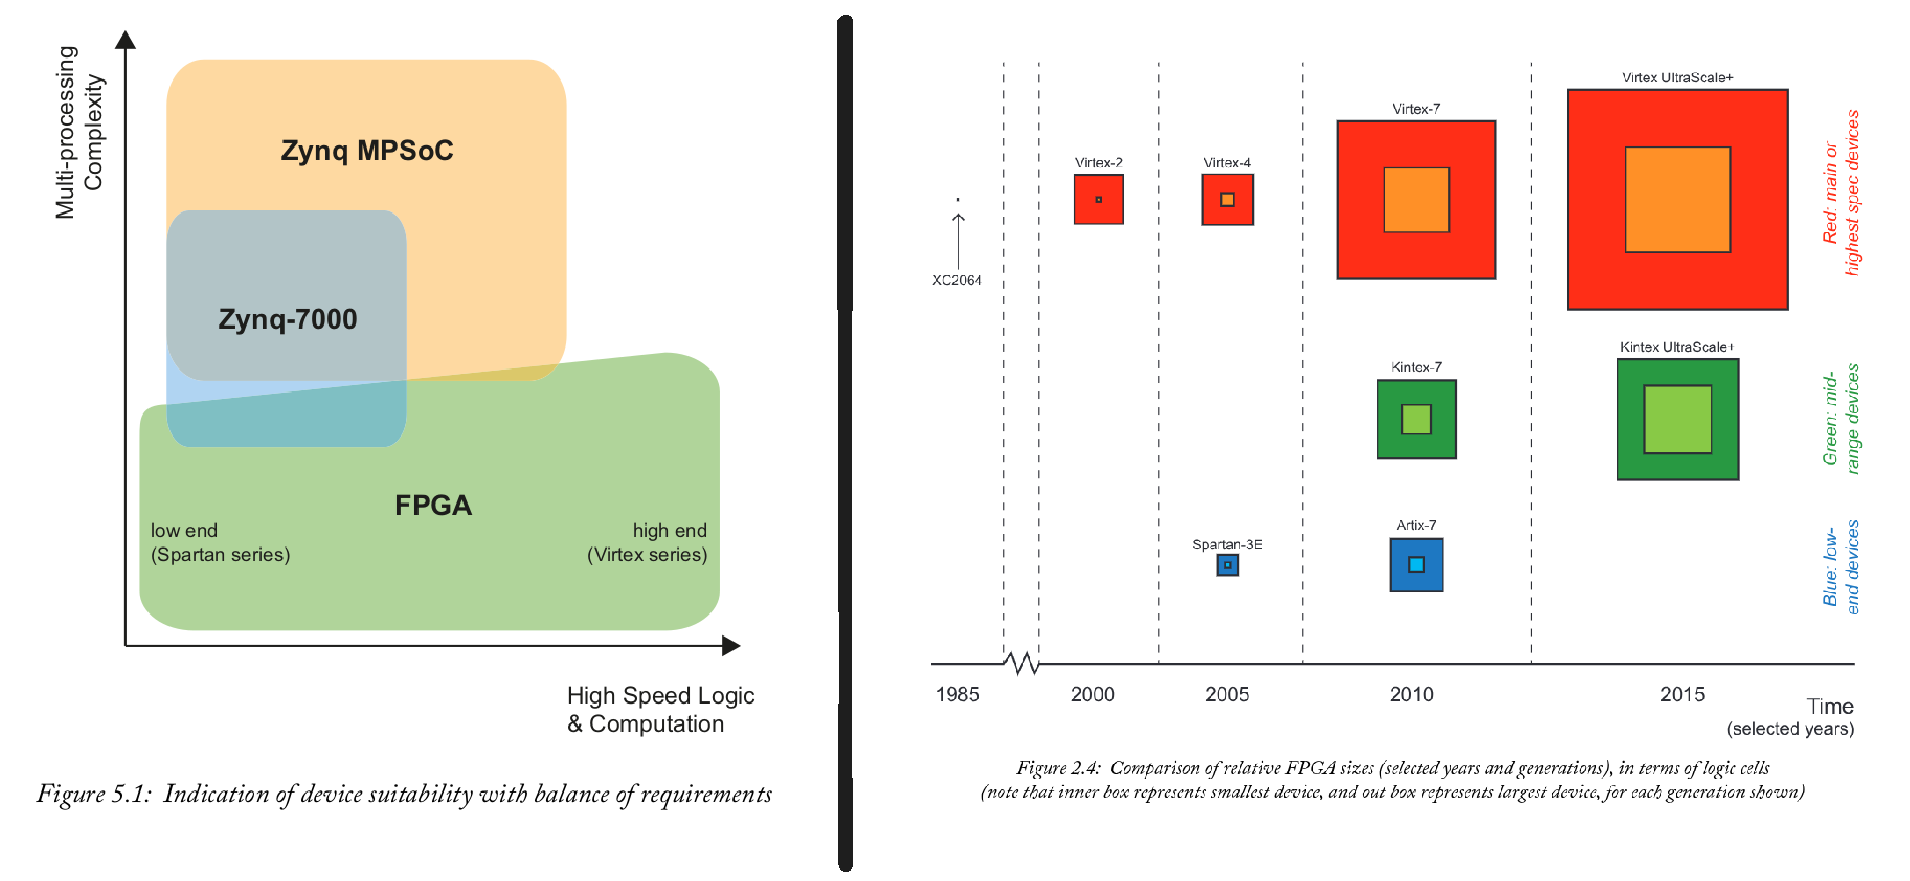
\includegraphics{cap2_familias_fpgas}
\caption[Elección de plataforma de HW programable y evolución de las FPGA]{%
(a)~Descripción cualitativa de la elección de plataforma de HW programable para
diferentes contextos de complejidad/\emph{performance}. (b)~Comparación del tamaño
relativo de los recursos lógicos de FPGA en años seleccionados.
\label{f:hw-familias-fpgas}}
\end{figure}

Es así que decidimos que la familia de placas de desarrollo Red Pitaya, que
contienen un SoC Zynq-7000, representa una buena plataforma de hardware para
este proyecto. A continuación se la describe en mayor detalle.

%%%%%%%%%%%%%%%%%%%%%%%%%%%%%%%%%%%%%%%%%%%%%%%%%%%%%%%%%%%%%%%%%%%%%%%%%%%%%%%%
\section{Plataforma empleada: Red Pitaya}
\label{S:hw-red-pitaya}

Una plataforma es un sistema especificado, con documentación y soporte, que
puede utilizarse como herramienta para resolver un problema. Nuestro proyecto
utiliza la Red Pitaya STEMlab 125-14; en la Fig.~\ref{f:hw-overview-pitaya} se
presenta una breve descripción de la placa. El chip cuadrado del centro, debajo
del disipador, es el SoC Zynq-7000: constituye el elemento central de
procesamiento de la plataforma, y a su alrededor están el resto de los
periféricos. Todos los modelos de Red Pitaya usan la misma familia de SoC,
Zynq-7000, pero no los mismos conversores ni el mismo front-end analógico
(Tabla~\ref{t:hw-modelos-pitaya}).

\begin{figure}[H]
\centering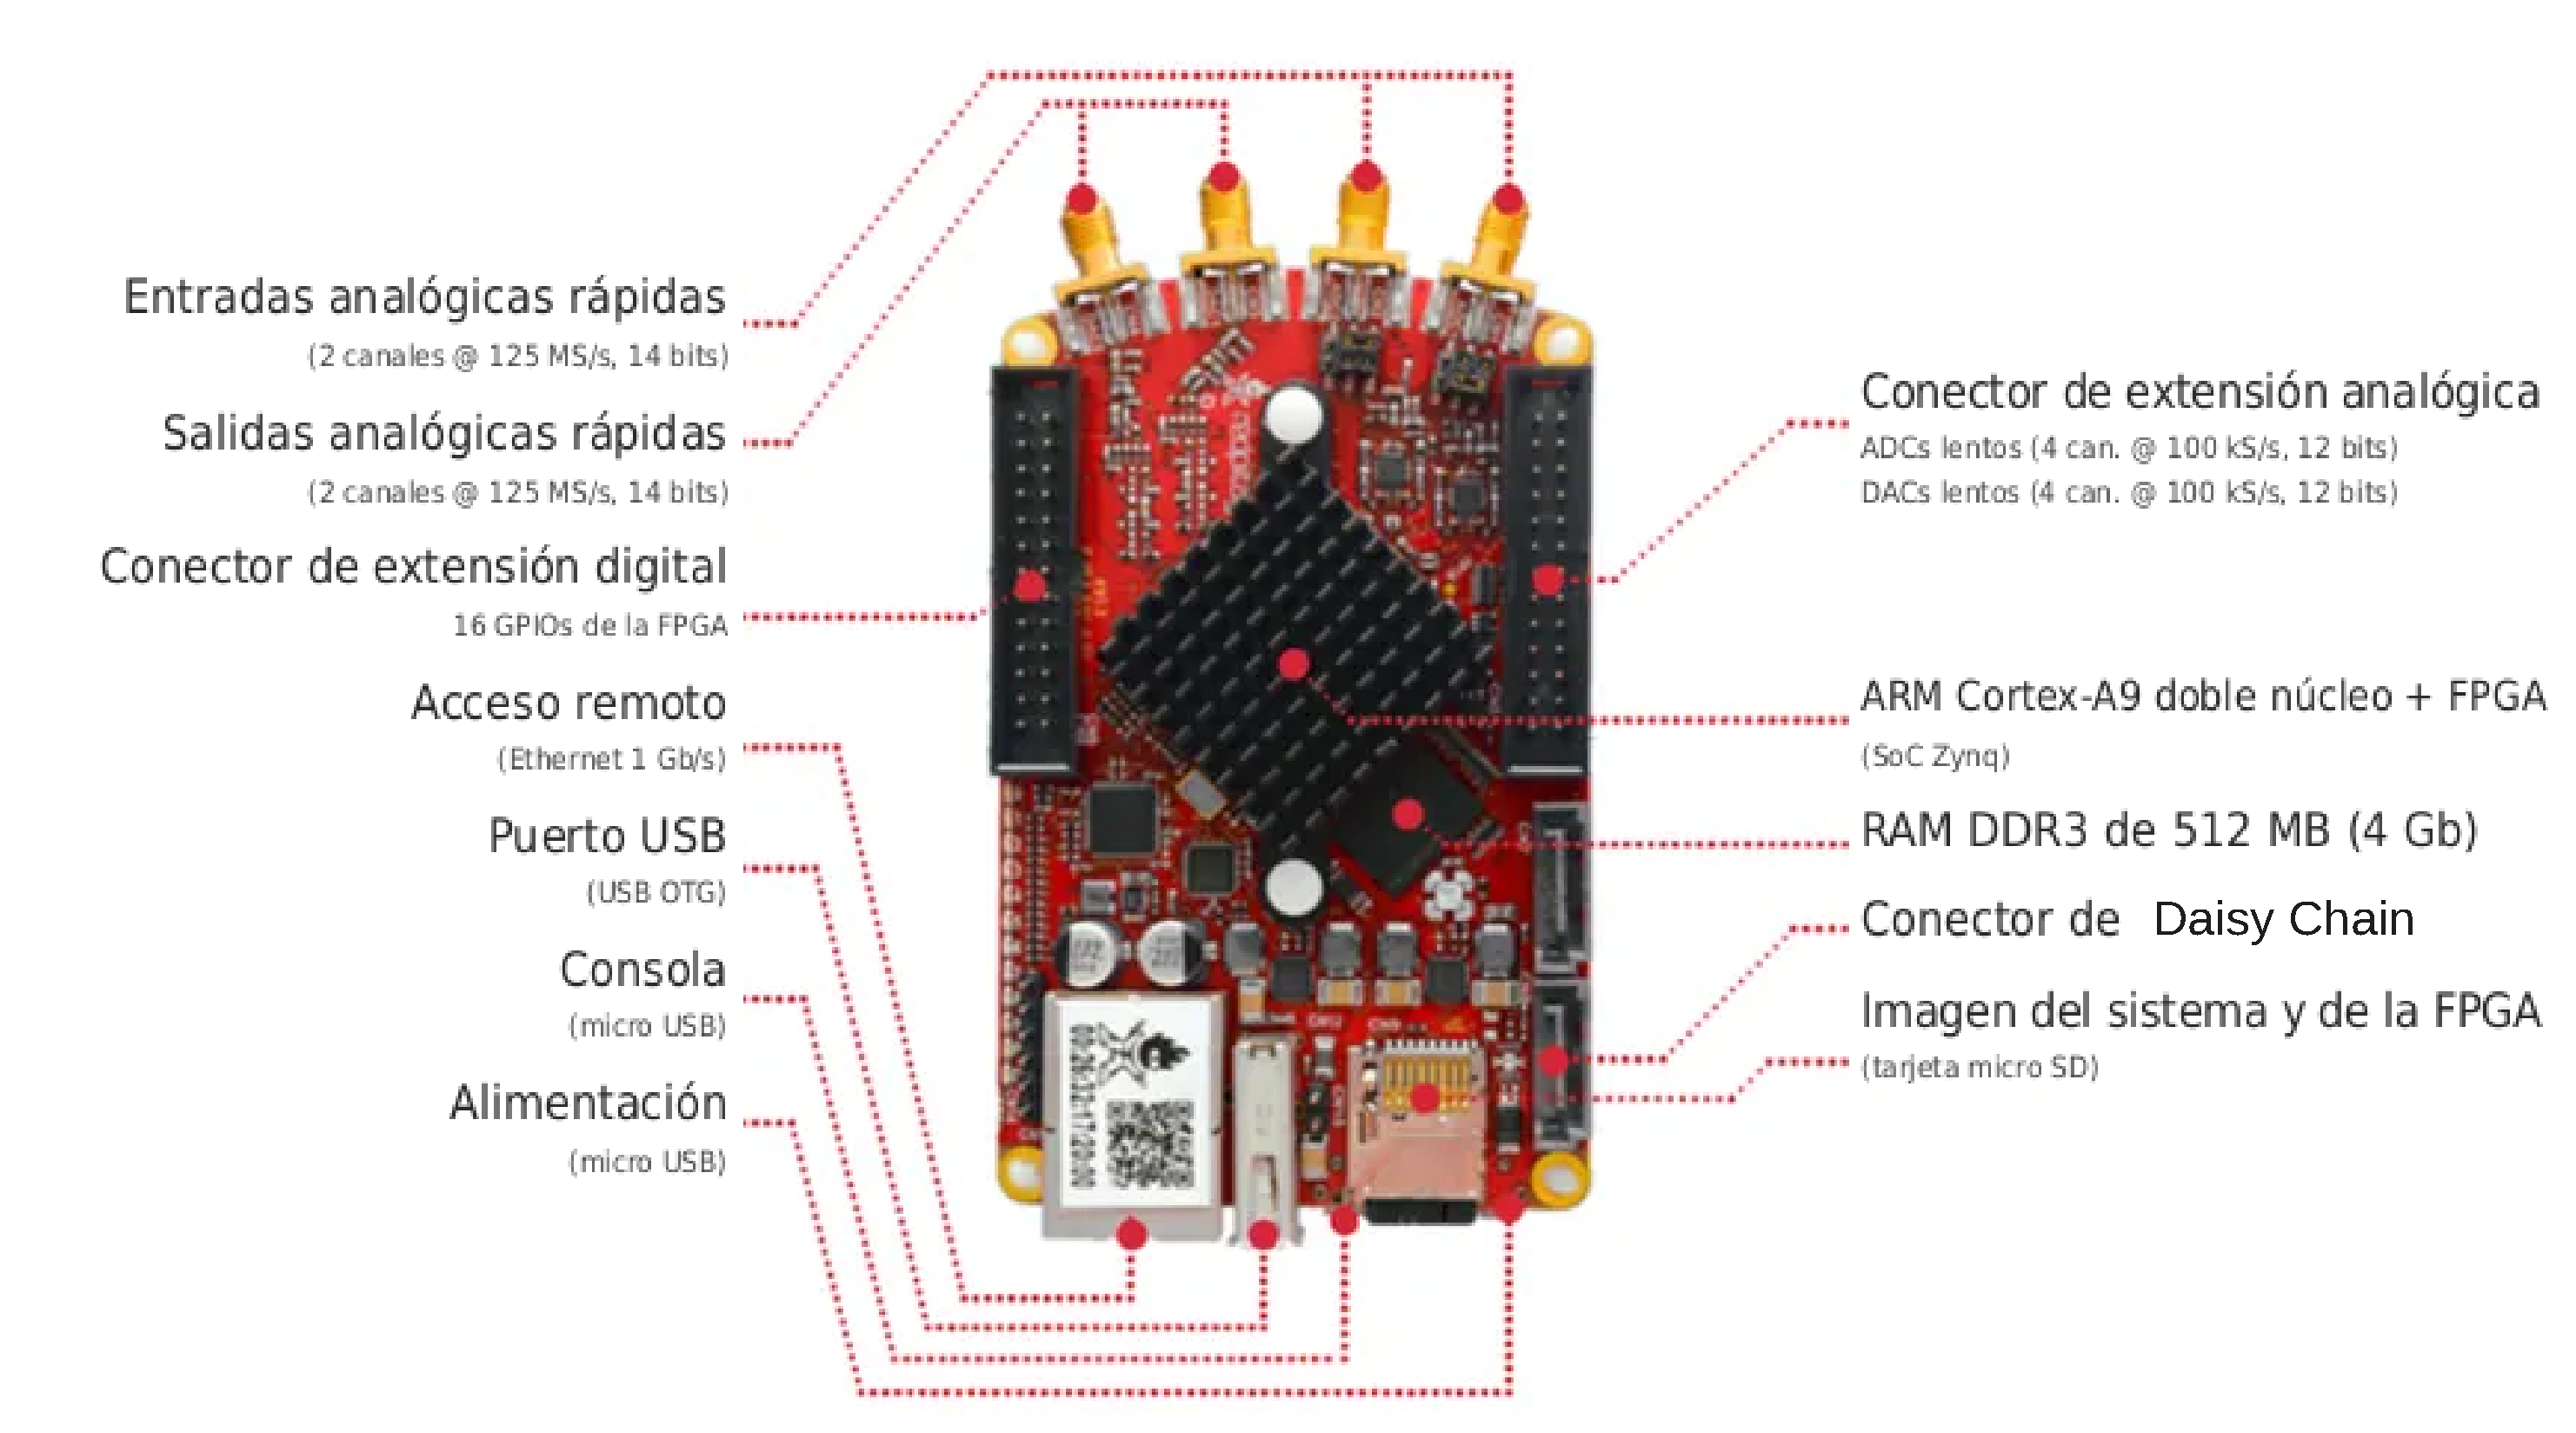
\includegraphics{cap2_overview_pitaya}
\caption[La placa STEMlab 125-14 y sus principales periféricos]{%
Foto de la placa de desarrollo STEMlab 125-14 y sus principales periféricos.
\label{f:hw-overview-pitaya}}
\end{figure}

Los principales cambios entre los modelos de Red Pitaya son los recursos de la
FPGA, las características del ADC, el tamaño de la RAM y la cantidad de
conectores digitales. En la Tabla~\ref{t:hw-modelos-pitaya} se presenta una
descripción general de las capacidades de las distintas placas.

\begin{table}[H]
\centering
\caption[Especificaciones de las placas Red Pitaya más comunes]{%
Especificaciones generales de las placas Red Pitaya más
comunes~\cite{RedPitayaDocs}.\label{t:hw-modelos-pitaya}}
\footnotesize
\setlength{\tabcolsep}{3pt}
\newcolumntype{Y}{>{\centering\arraybackslash}X}
\begin{tabularx}{\textwidth}{|>{\raggedright\arraybackslash}p{0.165\textwidth}|Y|Y|Y|Y|Y|Y|}
\hline
\encabezado \textbf{Característica} & \textbf{STEMlab 125-10}
  & \textbf{STEMlab 125-14} & \textbf{STEMlab 125-14 Z7020}
  & \textbf{STEMlab 125-14 4-Input} & \textbf{SDRlab 122-16}
  & \textbf{SIGNALlab 250-12} \\ \hline
SoC & Zynq 7010 & \textbf{Zynq 7010} & Zynq 7020 & Zynq 7020 & Zynq 7020
  & Zynq 7020 (grado -3) \\ \hline
RAM DDR3 & 256~MB & \textbf{512~MB} & 512~MB & 512~MB & 512~MB & 1~GB \\ \hline
ADC & 2~$\times$ 10 bit & \textbf{2~$\times$ 14 bit} & 2~$\times$ 14 bit
  & \textbf{4~$\times$ 14 bit} & 2~$\times$ 16 bit & 2~$\times$ 12 bit \\ \hline
Tasa ADC & 125~MS/s & \textbf{125~MS/s} & 125~MS/s & 125~MS/s & 122.88~MS/s
  & 250~MS/s \\ \hline
Ancho de banda & DC--50~MHz & \textbf{DC--60~MHz} & DC--60~MHz & DC--60~MHz
  & 300~kHz--550~MHz (AC) & DC--60~MHz \\ \hline
Rango de entrada & ±1~V / ±20~V & \textbf{±1~V / ±20~V} & ±1~V / ±20~V
  & ±1~V / ±20~V & 0.5~Vpp (50~$\Omega$) & ±1~V / ±20~V \\ \hline
DAC & 2~$\times$ 10 bit & \textbf{2~$\times$ 14 bit} & 2~$\times$ 14 bit & ---
  & 2~$\times$ 14 bit & 2~$\times$ 14 bit \\ \hline
Tasa DAC & 125~MS/s & \textbf{125~MS/s} & 125~MS/s & --- & 122.88~MS/s
  & 250~MS/s \\ \hline
GPIO (E1) & 16 & \textbf{16} & 22 & 22 & 22 & 19 \\ \hline
Ethernet & 1~Gbit & \textbf{1~Gbit} & 1~Gbit & 1~Gbit & 1~Gbit & 1~Gbit \\ \hline
USB & USB-A 2.0 & \textbf{USB-A 2.0} & USB-A 2.0 & USB-A 2.0 & USB-A 2.0
  & 2~$\times$ USB-A 2.0 \\ \hline
Alimentación & 5~V, 1.5~A & \textbf{5~V, 2~A} & 5~V, 2~A & 5~V, 2~A & 5~V, 2~A
  & 24~V, 0.5~A \\ \hline
Temperatura & 0--55~°C & \textbf{0--55~°C} & 0--55~°C & 0--55~°C & 0--55~°C
  & 0--55~°C \\ \hline
\end{tabularx}
\end{table}

En la Sec.~\ref{S:hw-perifericos} se describen en detalle los periféricos; vamos
a arrancar describiendo al protagonista del sistema en la Sec.~\ref{S:hw-soc}.

%%%%%%%%%%%%%%%%%%%%%%%%%%%%%%%%%%%%%%%%%%%%%%%%%%%%%%%%%%%%%%%%%%%%%%%%%%%%%%%%
\section{Arquitectura SoC: FPGA + µC}
\label{S:hw-soc}

Cuando se requería un hilo de trabajo secuencial y programable en una FPGA, se
sintetizaba un procesador sobre su \emph{fabric}. Estos procesadores se denominan
\emph{softcore} porque se construyen con los bloques maleables del \emph{fabric}; su
contrapunto son los \emph{hardcore}, implementados como ASIC, con una
funcionalidad completamente fijada por el fabricante.

Antes de que el procesador viniera integrado en el mismo chip, los softcores
eran la forma habitual de agregarle uno a una FPGA, y se siguen usando
(MicroBlaze~\cite{UG984}, Nios, núcleos RISC-V) para las siguientes actividades:
\begin{itemize}
  \item Lógica lenta pero de muchos pasos y ramificaciones.

    El ejemplo típico es cuando tenemos una tarea que requiere un algoritmo
    recursivo, es común resolver esto mediante la creación de un \emph{stack} dedicado
    por módulo, esto tiene la contra de que tenemos una región de memoria de uso
    extremadamente bajo y probablemente reducida para el trabajo de la tarea. Un
    CPU podría hacer uso de una memoria compartida, como es una RAM de forma de
    no tener estas limitaciones.
  \item Iterar sin re-sintetizar.
  \item Configurabilidad e instrucciones \emph{custom}.
  \item Múltiples \emph{cores} dedicados.
\end{itemize}

Esto nos dice algo muy importante de la estructura del HW, siempre que queremos
un elemento de control lo podemos sintetizar de manera independiente. Y esto
ocurre muy a menudo, por ejemplo cuando necesitamos mover datos en grandes
cantidades paquetes y de manera no continua se define un subsistema de memoria
llamado DMA, \emph{Direct Memory Access}, el cual toma el rol del CPU pero para
transferencias de datos. Este sería un acelerador pero de transferencia de
datos.

El problema principal de los softcores es el rendimiento. En la
Fig.~\ref{f:hw-softcore}(b) se compara el rendimiento del \textbf{mejor caso} de
tres familias de procesadores: en rosa el ARM Cortex-A9, el presente en este
trabajo; en gris el PowerPC de la Virtex-5, un procesador duro embebido en el
\emph{fabric}; y en azul oscuro tres softcores. Entre 2002 y 2010 hubo varias FPGA con
procesadores duros de este tipo (PowerPC 405 y 440 en las Virtex-II
Pro~\cite{DS083}, Virtex-4 FX y Virtex-5 FXT~\cite{UG200}); el Zynq-7000 (2011)
fue un paso más, con un sistema de procesamiento completo en el mismo chip.

\begin{figure}[H]
\centering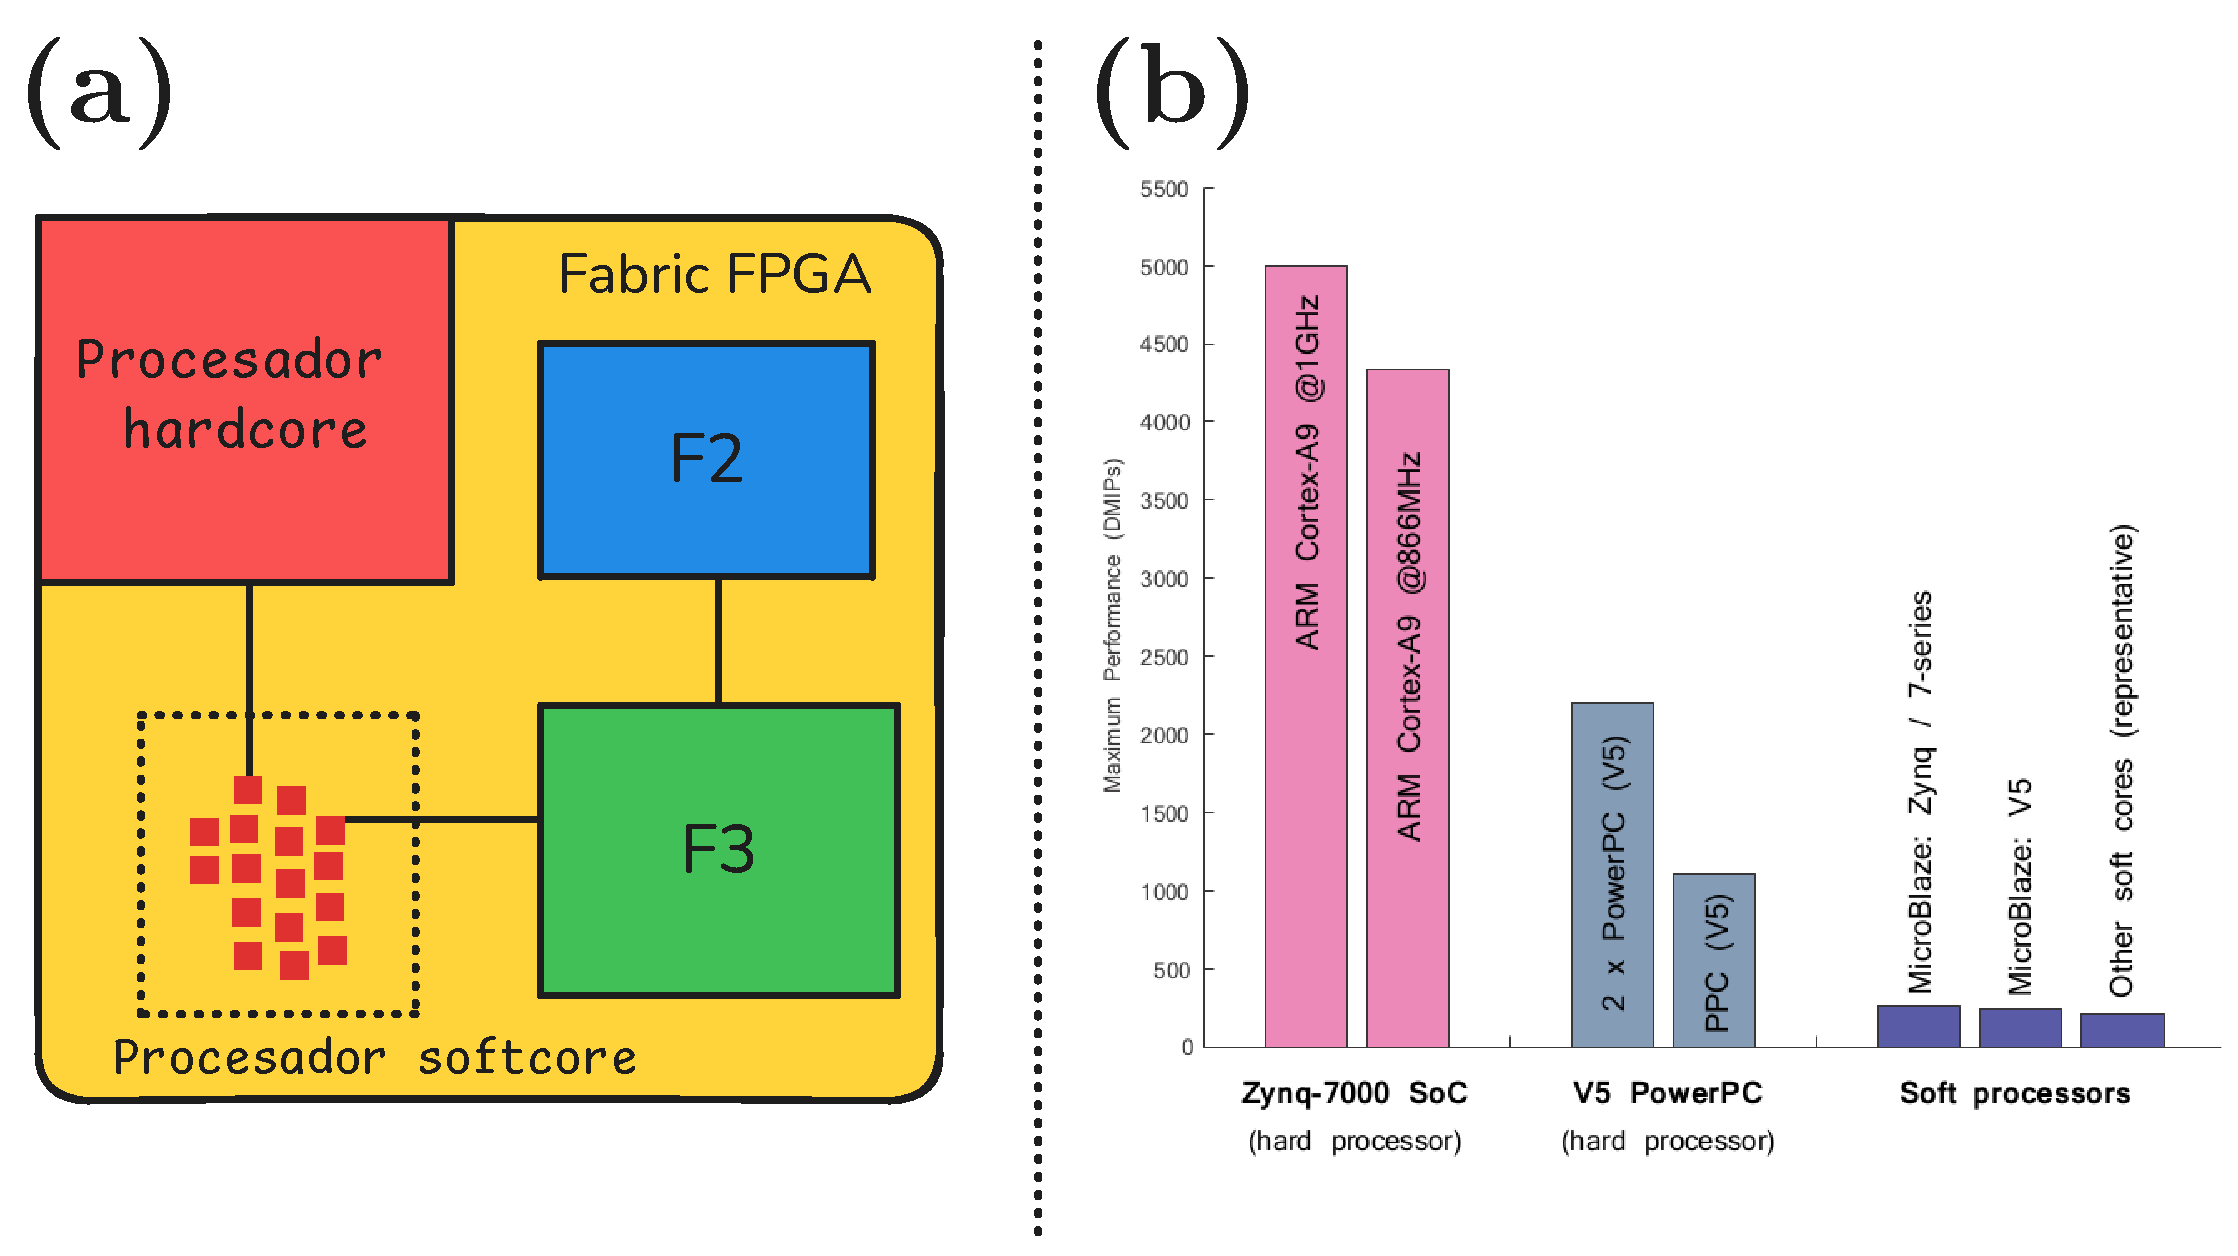
\includegraphics{cap2_softcore_hardcore}
\caption[Procesadores softcore y hardcore]{%
Comparación de procesadores softcore y hardcore. (a)~Comparación dentro de un
SoC: el procesador hardcore tiene su propia región del chip, dedicada e
inmodificable, y el procesador softcore ocupa lugar de la \emph{fabric} al lado de
otros módulos de HW, F2 y F3. (b)~Rendimiento máximo, en DMIPS
(\emph{Dhrystone millions of instructions per second}, un \emph{test} estandarizado de
\emph{performance}~\cite{Weicker1984}), de procesadores hardcore ---el Cortex-A9 del PS
del Zynq-7000, en rosa, y el PowerPC embebido en el \emph{fabric} de la Virtex-5, en
gris--- contra procesadores softcore instanciados en la PL, en azul oscuro.
Valores indicativos, del mejor caso. Extraída del
ZynqBook~\citefig{Crockett2014}{4.3}.\label{f:hw-softcore}}
\end{figure}

El punto a notar es que el Cortex-A9 doble rinde, en el mejor caso, entre 16 y
24 veces lo que un softcore; los dos núcleos de la placa, a 667~MHz, rinden unas
12 veces lo que un MicroBlaze. Un softcore con MMU, como el MicroBlaze, también
puede correr Linux~\cite{UG984}: lo que cambia con el hardcore es el
rendimiento, que alcanza para que nuestro sistema deje de trabajar como un
embebido y comience a funcionar como una computadora dedicada, con un sistema
operativo completo.

\subsection{Arquitectura del Zynq-7000}
\label{S:hw-zynq}

Aun siendo los dos sistemas de procesamiento, sus características son
extremadamente diferentes. Con el tiempo se vio el beneficio de acortar el
enlace entre ambos, y terminaron en el mismo encapsulado. Al estar en un mismo
chip cambió la forma típica de uso, y se les dieron nuevos nombres: la FPGA pasó
a llamarse \emph{programmable logic} (PL) y el procesador, \emph{processing
system} (PS)~\cite{UG585}.

\begin{figure}[H]
\centering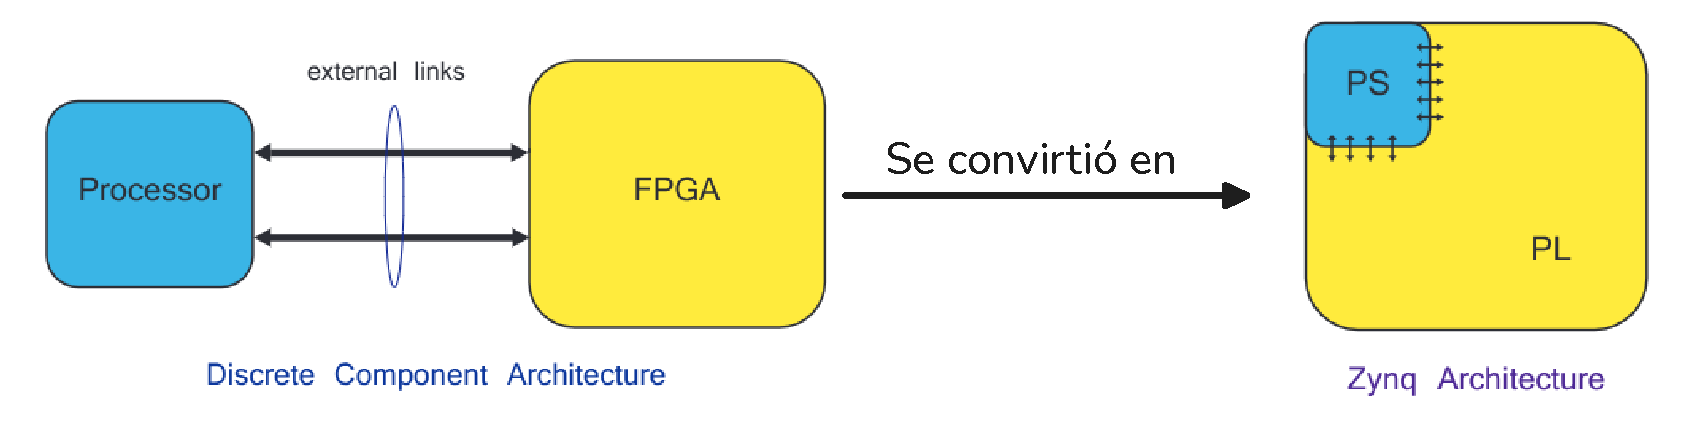
\includegraphics{cap2_arquitectura_zynq}
\caption[Combinación de procesador y FPGA]{%
Combinación de procesador + FPGA con enlaces externos a un chip.
\label{f:hw-arquitectura-zynq}}
\end{figure}

Los diferentes periféricos y módulos se conectan a una \textbf{red de
direccionamiento} interna del sistema llamada \emph{interconnect}, cuyo
funcionamiento es análogo al de los \emph{switches} de una red de computadoras: su
objeto es almacenar temporalmente (\emph{buffer}) y redireccionar las
transacciones para que la comunicación en el sistema sea eficiente. El
direccionamiento se hace mediante \textbf{direcciones}: cada módulo está
\textbf{mapeado en memoria}, es decir, tiene un conjunto de direcciones fijas.
Estas direcciones corresponden a registros clave expuestos al exterior, que
generalmente se llaman de \textbf{control} o de \textbf{estado}.

Todo lo que trabaje con el protocolo del \emph{interconnect} se puede conectar, y eso
es parte de su capacidad de extensión: generalmente se lo define con capacidad
para N conexiones esclavas y M maestras. En la
Fig.~\ref{f:hw-interconexiones-soc} se presentan distintos tipos de periféricos,
procesadores y memorias que comparten el mismo tipo de \emph{interconnect}.

\begin{figure}[H]
\centering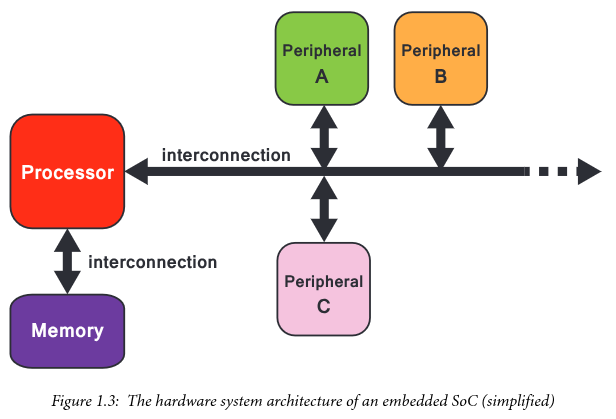
\includegraphics{cap2_interconexiones_soc}
\caption[Representación de un SoC]{%
Representación de un SoC. Extraído del ZynqBook~\cite{Crockett2014}.
\label{f:hw-interconexiones-soc}}
\end{figure}

El procesador principal en este proyecto es la PL así que vamos a comenzar
describiendo sus características, recursos e interfaces externas.

\subsection{Arquitectura de la lógica programable (PL)}
\label{S:hw-pl}

Parte de la potencia de la FPGA es su flexibilidad, que se obtiene mediante la
\textbf{configuración de los recursos lógicos programables}. En la
Tabla~\ref{t:hw-recursos-pl} se presentan los recursos de los dos Zynq de la
familia Red Pitaya.

\begin{table}[H]
\centering
\caption[Recursos lógicos de los Zynq de las placas Red Pitaya]{%
Recursos lógicos de los dos Zynq presentes en las placas Red
Pitaya~\cite{DS190}.\label{t:hw-recursos-pl}}
\small
\begin{tabular}{|l|r|r|c|}
\hline
\encabezado \textbf{Recurso de la PL} & \textbf{XC7Z010} & \textbf{XC7Z020}
  & \textbf{$\times$} \\ \hline
Celdas lógicas (unidad comercial, $\approx$ 1,6 LUT6) & 28\,k & 85\,k & 3.0 \\ \hline
CLB & 2\,200 & 6\,650 & 3.0 \\ \hline
\emph{Slices} (2 por CLB) & 4\,400 & 13\,300 & 3.0 \\ \hline
LUT6 & 17\,600 & 53\,200 & 3.0 \\ \hline
Flip-flops & 35\,200 & 106\,400 & 3.0 \\ \hline
Block RAM (RAMB36) & 60 (2.1~Mb) & 140 (4.9~Mb) & 2.3 \\ \hline
DSP48E1 & 80 & 220 & 2.75 \\ \hline
PLL / MMCM & 2 / 2 & 4 / 4 & 2 \\ \hline
\end{tabular}
\end{table}

El bloque básico del tejido lógico es el \textbf{\emph{Configurable Logic Block}
(CLB)}~\cite{UG474}. Cada CLB contiene \textbf{dos \emph{slices}} y se conecta
al resto del dispositivo a través de una \textbf{matriz de conmutación}
(\emph{switch matrix}), que es su único acceso a la red de interconexión
general; en la Sec.~\ref{S:ap-hw-clb} se describen más detalles. Estos
bloques están distribuidos por el cuerpo de la FPGA. En la
Fig.~\ref{f:hw-bloques-fpga}(b) se ve el \emph{fabric} en forma de L: la esquina
faltante del rectángulo del die la ocupa físicamente el PS. El tejido está
organizado en filas y columnas de dimensiones cuantizadas; dentro de esa grilla
se colocan bloques del mismo tipo a lo largo de columnas enteras (una columna de
CLB, una columna de Block RAM, una columna de DSP), y las columnas están
separadas por canales de interconexión a los que se accede por las matrices de
conmutación.

\begin{figure}[H]
\centering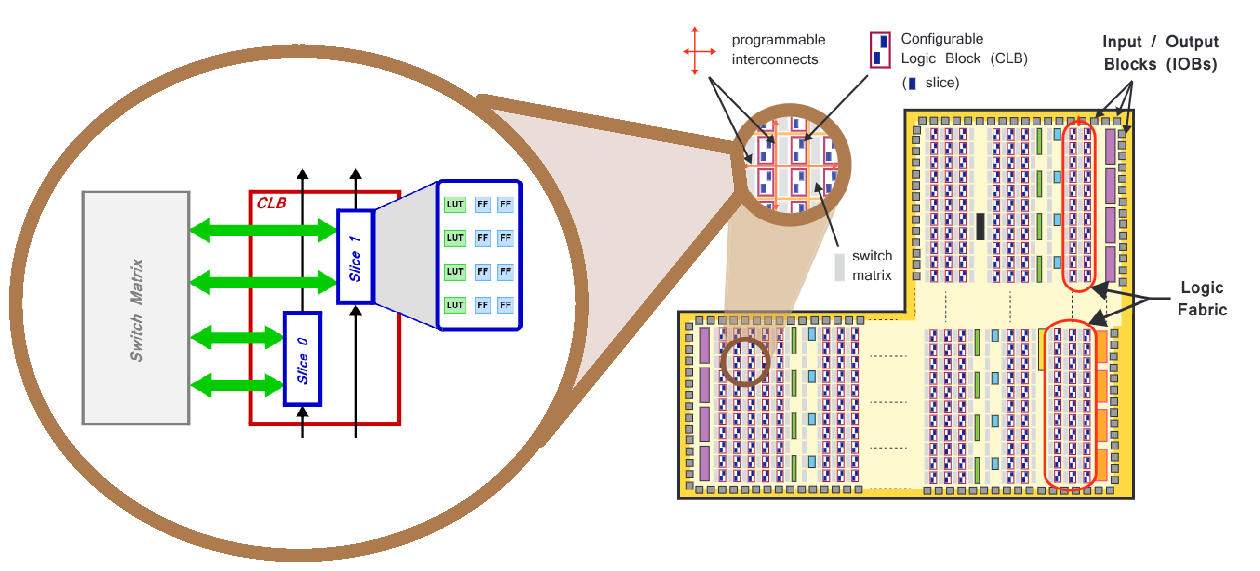
\includegraphics{cap2_bloques_basicos_fpga}
\caption[Bloques básicos de la FPGA]{%
Bloques básicos de la FPGA. (a)~Composición elemental de una CLB. (b)~\emph{Fabric}
del Zynq7010 y sus elementos constitutivos básicos. Estos incluyen las CLBs y
interconexiones programables.\label{f:hw-bloques-fpga}}
\end{figure}

Además del \emph{fabric} genérico, la arquitectura incorpora bloques duros
(\emph{hard macros}), optimizados para funciones que serían caras de construir
con LUT, en la Tabla~\ref{t:hw-hardmacros} se presentan las que se utilizaron
para este proyecto.

\begin{table}[H]
\centering
\caption[Hardmacros especializadas dentro de la PL del Zynq]{%
Hardmacros especializadas dentro de la PL del
Zynq~\cite{UG473,UG479,UG472,UG471,UG480}.\label{t:hw-hardmacros}}
\small
\begin{tabularx}{\textwidth}{|>{\raggedright\arraybackslash}p{0.17\textwidth}|>{\raggedright\arraybackslash}X|>{\raggedright\arraybackslash}p{0.2\textwidth}|}
\hline
\encabezado \textbf{Recurso} & \textbf{Qué es} & \textbf{Presentes en XC7Z010} \\ \hline
\textbf{Block RAM} & Memorias de 36~Kb, divisibles en dos de 18~Kb, de
  \textbf{doble puerto verdadero}, con ancho de palabra configurable y modo FIFO
  integrado & 60 bloques (2.1~Mb) \\ \hline
\textbf{DSP48E1} & Pre-sumador + multiplicador con signo de \textbf{25~$\times$
  18 bits} + acumulador de 48 bits, encadenables entre sí sin pasar por el
  tejido & 80 \\ \hline
\textbf{\emph{Clock tiles} (CMT)} & gestión de reloj: MMCM y PLL, que sintetizan,
  multiplican y desfasan relojes & 2 MMCM + 2 PLL \\ \hline
\textbf{\emph{Buffers} de reloj} & BUFG (red global), BUFH (regional), BUFR/BUFIO (de
  entrada/salida) & 32 BUFG, 48 BUFH, 8 BUFR, 8 BUFIO \\ \hline
\textbf{IOB} & bloques de entrada/salida, con registros propios
  (ILOGIC/OLOGIC), serializadores (ISERDES/OSERDES), dobladores de tasa
  (IDDR/ODDR) y líneas de retardo calibradas (IDELAY) & 100 pines utilizables
  \\ \hline
\textbf{XADC} & ADC de 12 bits y 1~MS/s integrado, con sensores internos de
  temperatura y tensión & 1 \\ \hline
\end{tabularx}
\end{table}

En nuestra aplicación usamos tanto los recursos de entrada a la PL, con las
conexiones del ADC, como los de salida de la PL, con la conexión al PS. Se
describen en la Sec.~\ref{S:hw-interconexiones}.

\subsection{Interconexiones presentes}
\label{S:hw-interconexiones}

En la Fig.~\ref{f:hw-interfaces-zynq}(a) se presenta buena parte de las
interconexiones internas y externas del Zynq-7010. Las más importantes para este
proyecto son las interfaces AXI (\emph{Advanced eXtensible Interface}), las
principales entre el PS y la PL. AXI es una familia de estándares
AMBA~\cite{AMBAAXI} de \textbf{buses intrachip} de \textbf{alta \emph{performance}} y
de tipo \textbf{punto a punto}. En la Fig.~\ref{f:hw-interfaces-zynq}(b) se
presentan las nueve interfaces AXI del sistema, que se dividen en tres grupos:
\emph{general purpose} (GP), \emph{high performance} (HP) y \emph{accelerator
coherency port} (ACP).

\begin{figure}[H]
\centering
\begin{minipage}[b]{0.56\textwidth}\centering
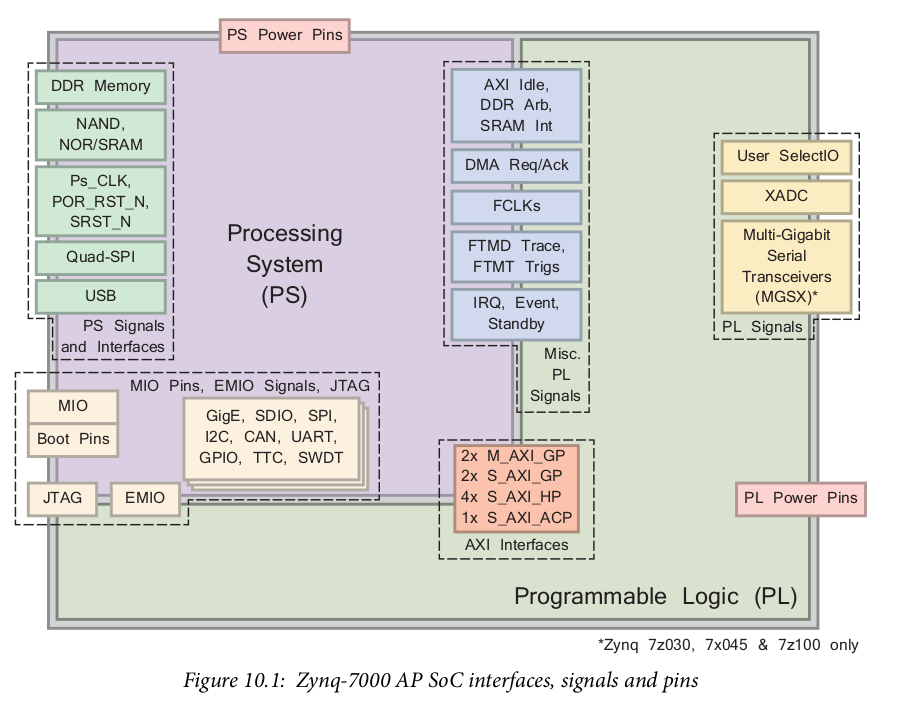
\includegraphics[width=\linewidth]{cap2_interfaces_zynq}\\(a)
\end{minipage}\hfill
\begin{minipage}[b]{0.42\textwidth}\centering
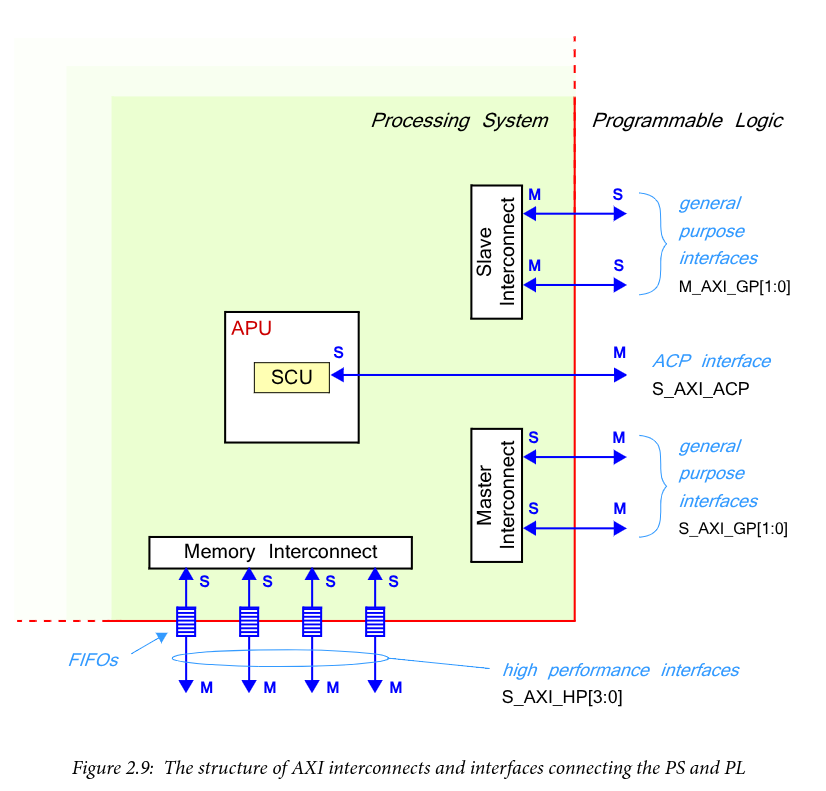
\includegraphics[width=\linewidth]{cap2_interfaces_axi}\\(b)
\end{minipage}
\caption[Interfaces del SoC e interfaces AXI entre el PS y la PL]{%
(a) Interfaces internas y externas del SoC. Extraído del
ZynqBook~\citefig{Crockett2014}{10.1}. (b) Interfaces AXI entre el PS y la PL
del SoC, descritas en detalle en la Tabla~\ref{t:hw-axi}.\label{f:hw-interfaces-zynq}}
\end{figure}

Las características principales de cada una se describen en la
Tabla~\ref{t:hw-axi}. Las mayores diferencias son el \textbf{\emph{throughput} máximo
obtenible}, la \textbf{latencia de acceso} y la cantidad de conexiones
disponibles.

\begin{table}[H]
\centering
\caption[Propiedades de las interconexiones AXI entre el PS y la PL]{%
Propiedades de las interconexiones AXI entre el PS y la PL~\cite{UG585}. El
esclavo de Red Pitaya está en su repositorio~\cite{RedPitayaFPGA}.
\label{t:hw-axi}}
\footnotesize
\setlength{\tabcolsep}{3pt}
\newcolumntype{Y}{>{\raggedright\arraybackslash}X}
\begin{tabularx}{\textwidth}{|>{\raggedright\arraybackslash}p{0.13\textwidth}|Y|Y|Y|Y|}
\hline
\encabezado & \codigo{M\_AXI\_GP} & \codigo{S\_AXI\_GP} & \codigo{S\_AXI\_HP}
  & \codigo{S\_AXI\_ACP} \\ \hline
\textbf{Ancho de bus} & 32 bit & 32 bit & \textbf{64 bit} (configurable 32/64)
  & 64 bit \\ \hline
\textbf{Techo teórico} & 32~b $\times$ 150~MHz = \textbf{600~MB/s} & 600~MB/s
  & 64~b $\times$ 150~MHz = \textbf{1200~MB/s} por puerto & 1200~MB/s \\ \hline
\textbf{Ráfagas} & las admite AXI, \textbf{pero el esclavo de Red Pitaya no}
  & sí & \textbf{sí}, hasta 16 \emph{beats}, con FIFO de lectura y de escritura
  & sí \\ \hline
\textbf{Caso de uso típico} & \textbf{registros de control y estado}; lecturas
  chicas y esporádicas & que la PL acceda a periféricos del PS u OCM
  & \textbf{volcado masivo a DDR}: captura de ADC, video, DMA
  & acelerador que comparte estructuras con el CPU sin invalidar caché \\ \hline
Cantidad disponibles & 2 & 2 & 4 & 1 \\ \hline
\end{tabularx}
\end{table}

Para conectar múltiples puntos entre sí con una topología modificable se suelen
utilizar IP dedicadas, los \emph{interconnects} de Xilinx~\cite{PG059}. La
versión más empleada es el \textbf{\emph{crossbar}}, que puede observarse en la
Fig.~\ref{f:hw-topologia}(a): tiene una forma ``matricial'', con filas, columnas
y un interruptor en cada intersección que conecta ese vértice; canalizando bien
las transacciones podemos conectar varios pares de elementos de forma
simultánea. En la Fig.~\ref{f:hw-topologia}(b) se presenta la topología
estrella, que necesita muchas menos trazas a nivel de silicio pero sólo puede
comunicar un par de puntos a la vez. Vamos a ver en la
Sec.~\ref{S:intro-hw-bus-custom} que Red Pitaya utiliza esta topología para su bus \emph{custom}.

\begin{figure}[H]
\centering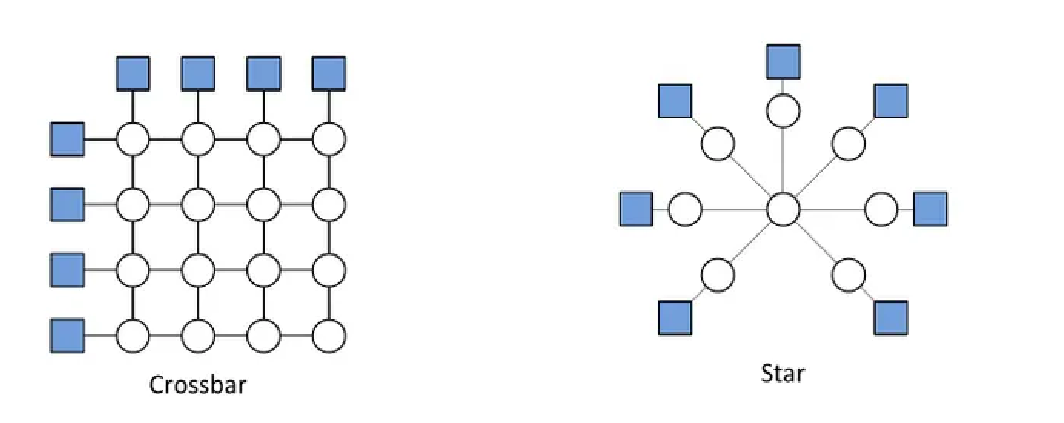
\includegraphics{cap2_topologia_interconnect}
\caption[Tipos de \emph{interconnects} más utilizados dentro del HW]{%
Tipos de \emph{interconnects} más utilizados dentro del HW. (a)~Interconexionado
\emph{crossbar}. (b)~Interconexionado estrella.\label{f:hw-topologia}}
\end{figure}

\subsection{Procesador Cortex-A9}
\label{S:hw-cortex-a9}

El Cortex-A9, anunciado en 2007, fue el núcleo de alta gama de la arquitectura
\textbf{ARMv7-A} (presentada en 2005 con el Cortex-A8) hasta la llegada del
Cortex-A15. Está diseñado para correr sistemas operativos
completos~\cite{DDI0388}. El Zynq-7010 de la placa trae \textbf{dos núcleos a
667~MHz} (grado de velocidad $-1$)~\cite{DS190}. La jerarquía de memoria del
procesador se presenta en la Fig.~\ref{f:hw-memoria-a9}.

\begin{figure}[H]
\centering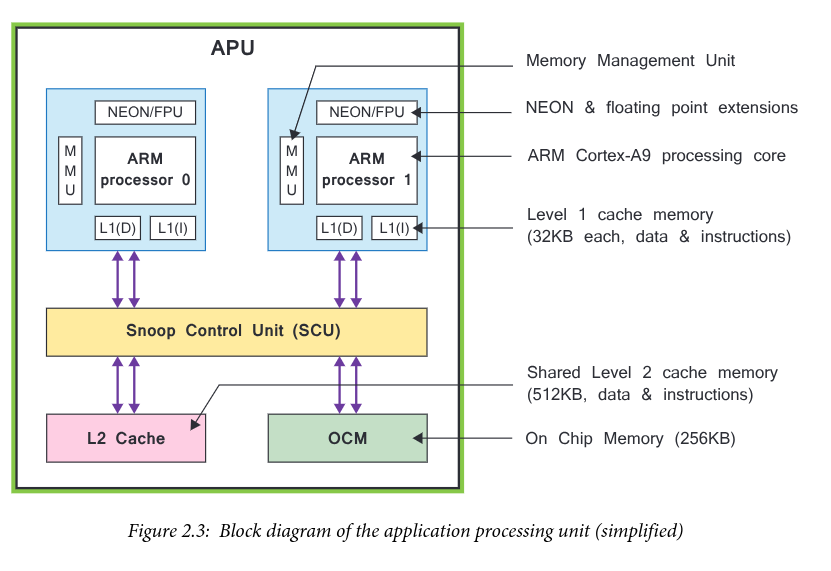
\includegraphics{cap2_jerarquia_memoria_a9}
\caption[Jerarquía de la memoria del APU]{%
Jerarquía de la memoria del APU.\label{f:hw-memoria-a9}}
\end{figure}

El tamaño de cada bloque condiciona en gran medida el rendimiento real. En orden
creciente de tamaño y de tiempo de acceso están la caché de nivel 1 (L1), la
caché de nivel 2 (L2), la memoria en chip (OCM) y la DDR3 externa; sus
características se presentan en la Tabla~\ref{t:hw-memorias}.

\begin{table}[H]
\centering
\caption[Niveles de memoria del PS del Zynq-7010]{%
Niveles de memoria del PS del Zynq-7010 en la STEMlab
125-14~\cite{UG585}.\label{t:hw-memorias}}
\small
\begin{tabularx}{\textwidth}{|l|l|>{\raggedright\arraybackslash}X|>{\raggedright\arraybackslash}X|}
\hline
\encabezado \textbf{Nivel} & \textbf{Tamaño} & \textbf{Organización}
  & \textbf{Alcance} \\ \hline
\textbf{L1 instrucciones} & 32~KB por núcleo & 4 vías & privado de cada núcleo \\ \hline
\textbf{L1 datos} & 32~KB por núcleo & 4 vías & privado de cada núcleo \\ \hline
\textbf{L2 unificada} & 512~KB & 8 vías (controlador PL310)
  & compartida por los dos núcleos \\ \hline
\textbf{OCM} & 256~KB & SRAM en el die, sin caché
  & los dos núcleos \textbf{y la PL} \\ \hline
\textbf{DDR3 externa} & 512~MB en esta placa & 16 bits a 533~MHz
  & $\sim$2.1~GB/s de pico teórico \\ \hline
\end{tabularx}
\end{table}

Cada núcleo tiene una \emph{memory management unit} (MMU)~\cite{DDI0406C}, que
traduce, página por página, las direcciones \textbf{virtuales} que usa el
software a las direcciones \textbf{físicas} que salen al bus. Sus tareas son:
\begin{enumerate}
  \item \textbf{Aislamiento}: cada \textbf{proceso} tiene su propio mapa de
    memoria virtual y no puede nombrar la memoria de otro proceso. Los dos
    núcleos, en cambio, comparten la memoria física y el mismo \emph{kernel}; por eso
    hace falta la SCU que se describe más abajo.
  \item \textbf{Eficiencia en el manejo de memoria}: el sistema operativo asigna
    la memoria en páginas, asocia cada región virtual contigua a páginas físicas
    que pueden estar dispersas y puede reubicarlas sin que el programa se
    entere.
  \item \textbf{Manejo de atributos por página}: cada página cuenta con banderas
    que determinan permisos (acceso: lectura/escritura/ejecución, y modo:
    usuario/privilegiado) y el \textbf{tipo de memoria}, esta categoría se
    explica en la Sec.~\ref{S:hw-modelo-memoria}.
\end{enumerate}

En este proyecto la MMU es el mecanismo por el cual el software llega a la PL:
abrir \ruta{/dev/mem} y hacer \codigo{mmap} de \codigo{0x4000\_0000} le pide a
la MMU una entrada de tabla que apunte a los registros de la PL, marcada como no
cacheable.

Mientras que la \emph{Snoop Control Unit} (SCU)~\cite{DDI0407}
\textbf{mantiene coherentes} las cachés L1 de datos de los dos núcleos, es
decir, garantiza que cada dirección de memoria tenga un único valor vigente.
Para lograrlo guarda una copia duplicada de los \emph{tags} de las dos L1: de forma que
sabe en todo momento qué líneas tiene cada núcleo, y así puede husmear
(\emph{snooping}) \textbf{sólo al que corresponde} en cada acceso conflictivo.
Qué accesos identifica el sistema como conflictivos depende del esquema de
coherencia por línea de caché, el más conocido es \textbf{MESI}
(\emph{Modified / Exclusive / Shared / Invalid}), para más info se refiere al
libro de Nagarajan et al.~\cite{Nagarajan2020}.

Su arquitectura de conjunto de instrucciones (ISA) es la combinación de
diferentes subconjuntos con objetivos específicos, presentados en la
Tabla~\ref{t:hw-isa}~\cite{DDI0406C}.

\begin{table}[H]
\centering
\caption[Conjuntos de instrucciones del Cortex-A9 y su uso en el proyecto]{%
Diferentes conjuntos de ISA estándares, la funcionalidad y criterio de diseño
empleados y la utilización de los mismos en el proyecto actual.
\label{t:hw-isa}}
\small
\begin{tabularx}{\textwidth}{|>{\raggedright\arraybackslash}p{0.17\textwidth}|>{\raggedright\arraybackslash}X|>{\raggedright\arraybackslash}X|}
\hline
\encabezado \textbf{Conjunto} & \textbf{Qué es}
  & \textbf{Utilización en el proyecto} \\ \hline
\textbf{ARM (A32)} & Instrucciones de 32 bits de ancho fijo, ejecución
  condicional en casi todas & Sólo si se compila con \codigo{-marm} \\ \hline
\textbf{Thumb-2} & mezcla de 16 y 32 bits: $\sim$30~\% menos código con
  rendimiento equivalente & El que genera gcc por defecto en armhf
  (Ubuntu/Debian)~\cite{DebianArmHF}: el código de Linux y el de este proyecto
  \\ \hline
\textbf{VFPv3} & unidad de punto flotante IEEE-754, simple y \textbf{doble}
  precisión, 32 registros de 64 bits & \codigo{double} de C, \codigo{float64}
  de NumPy \\ \hline
\textbf{NEON (Advanced SIMD)} & SIMD de 128 bits: 16 registros Q de 128 bits,
  alias de 32 registros D de 64. Enteros de 8/16/32/64 bits y flotante de
  \textbf{simple precisión} & Lo que vectoriza NumPy en float32 y en enteros;
  no en float64, su tipo por defecto, porque NEON de ARMv7 no tiene doble
  precisión \\ \hline
\textbf{TrustZone} & extensiones de seguridad, mundo seguro/no seguro & --- \\ \hline
\textbf{Jazelle / ThumbEE} & ejecución de bytecode, heredados y obsoletos
  & --- \\ \hline
\end{tabularx}
\end{table}

\subsection{Modelo de memoria}
\label{S:hw-modelo-memoria}

ARMv7 distingue tres \textbf{tipos de memoria}, y el tipo lo fija la tabla de
páginas de la \emph{Memory Management Unit} (MMU):

\begin{table}[H]
\centering
\caption[Modelo de memoria de ARMv7]{%
Modelo de memoria de ARMv7~\cite{DDI0406C}.\label{t:hw-modelo-memoria}}
\small
\begin{tabularx}{\textwidth}{|l|X|}
\hline
\encabezado \textbf{Tipo} & \textbf{Qué permite el procesador} \\ \hline
\textbf{Normal} & reordenar, fusionar, especular, cachear, leer de más
  (\emph{prefetch}) \\ \hline
\textbf{\emph{Device}} & sin reordenamiento entre accesos, sin fusión, sin
  especulación, sin acceso adelantado \\ \hline
\textbf{\emph{Strongly-ordered}} & como \emph{Device}, y además el acceso no se completa
  hasta llegar al destino \\ \hline
\end{tabularx}
\end{table}

Esto es importante porque los registros de la PL se acceden con un tipo de
memoria sin caché: \textbf{\emph{Device}} si los mapea un \emph{driver} del \emph{kernel}
(\codigo{ioremap}), y \textbf{\emph{Strongly-ordered}} si, como en este proyecto, se
mapean desde el espacio de usuario con \codigo{mmap} sobre
\ruta{/dev/mem}~\cite{LinuxMMU}. Ninguno de los dos tipos impide que el
compilador emita instrucciones de acceso múltiple
(\codigo{LDM}/\codigo{STM}) o de NEON: la arquitectura las permite, y en el bus
AXI se convierten en ráfagas o accesos anchos que el esclavo de Red Pitaya no
acepta. Si no lo tenemos en cuenta podemos tener problemas graves, como los
presentados en la Sec.~\ref{S:intro-hw-modos-falla}, que llegan hasta un reinicio completo
del sistema.

%%%%%%%%%%%%%%%%%%%%%%%%%%%%%%%%%%%%%%%%%%%%%%%%%%%%%%%%%%%%%%%%%%%%%%%%%%%%%%%%
\section{Periféricos externos a la Pitaya}
\label{S:hw-perifericos}

Para describirlos nos referimos al diagrama en bloques de la placa, presentado
en la Fig.~\ref{f:hw-diagrama-bloques}.

\begin{figure}[H]
\centering
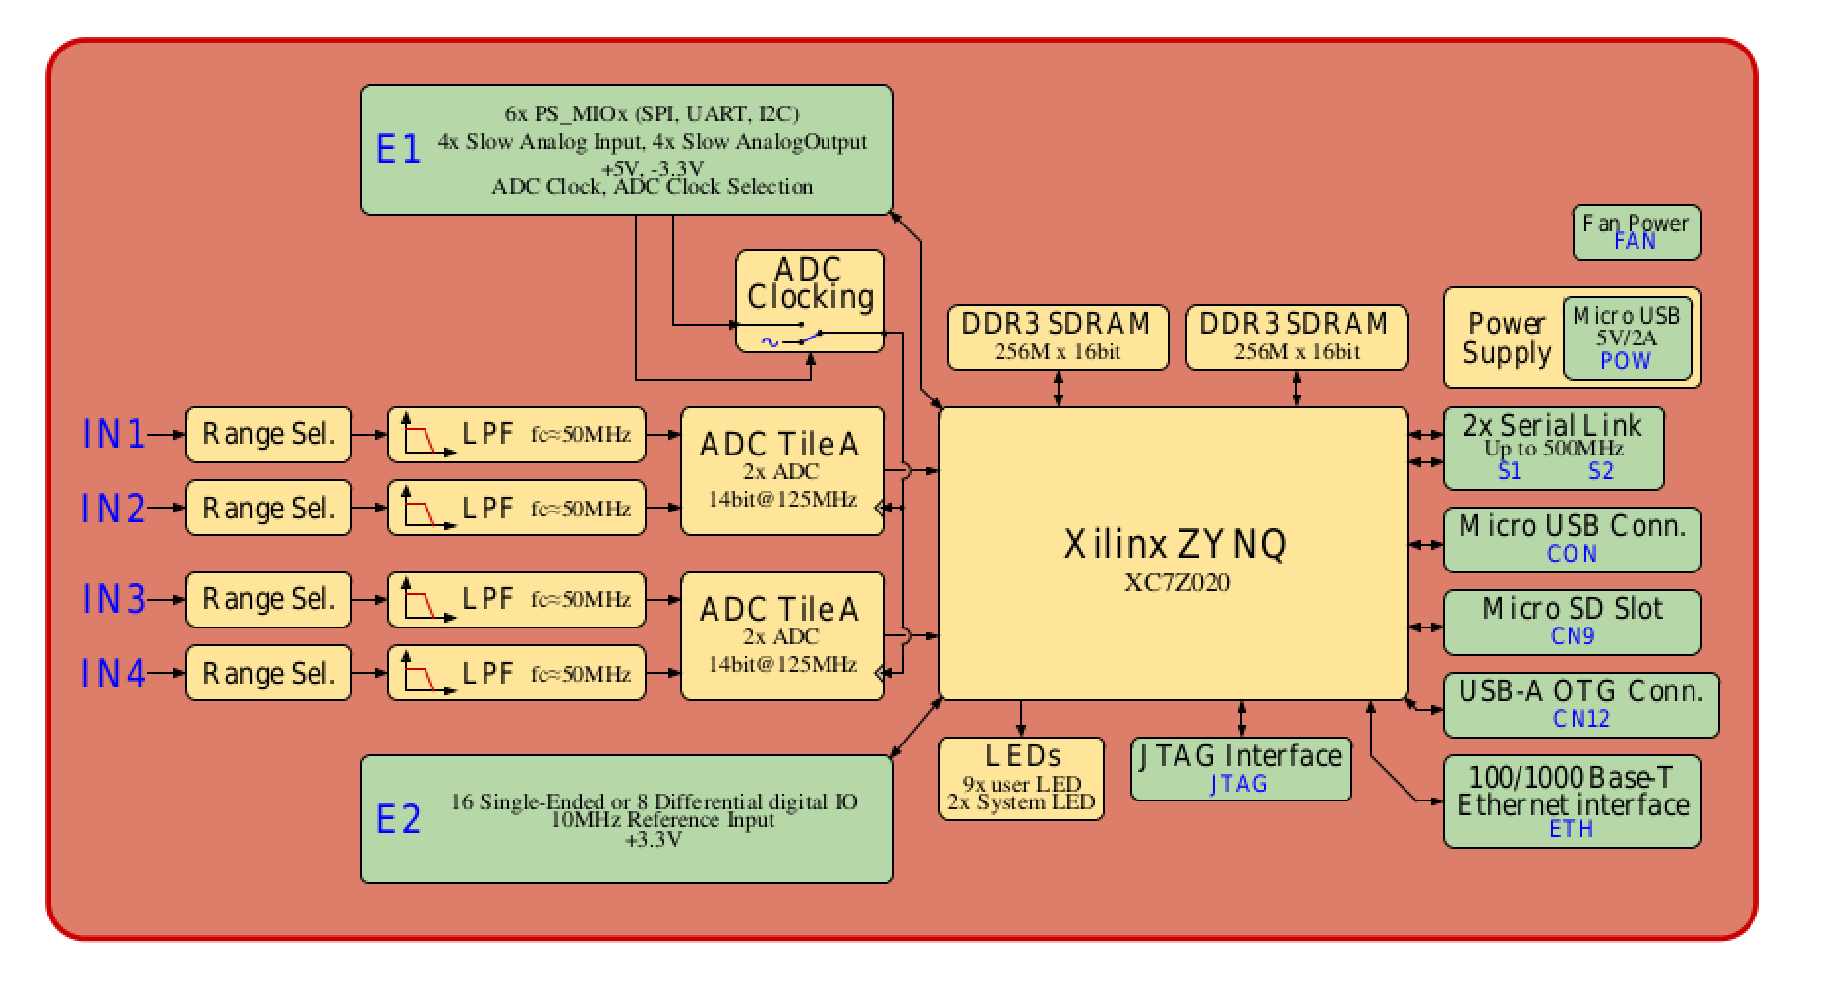
\includegraphics{cap2_diagrama_bloques_pitaya}
\caption[Diagrama de bloques de la plataforma]{%
Diagrama de bloques de la plataforma.\label{f:hw-diagrama-bloques}}
\end{figure}

\subsection{Entrada analógica presente: ADC}
\label{S:hw-adc}

La señal digitalizada es la base del procesamiento en todo el dispositivo. La
STEMlab 125-14 (y sus variantes Z7020 y 4-Input) usa el conversor
analógico-digital (ADC) LTC2145-14 de Analog Devices~\cite{LTC2145}; los otros
modelos cambian de conversor (Tabla~\ref{t:hw-modelos-pitaya}). Sus
características principales se presentan en la Tabla~\ref{t:hw-ltc2145}.

\begin{table}[H]
\centering
\caption[Características del ADC LTC2145-14 y del front-end de entrada]{%
Características principales del ADC LTC2145-14 y del front-end de entrada de la
STEMlab 125-14~\cite{LTC2145,RedPitayaDocs}.\label{t:hw-ltc2145}}
\small
\begin{tabularx}{\textwidth}{|>{\raggedright\arraybackslash}p{0.25\textwidth}|>{\raggedright\arraybackslash}X|}
\hline
\encabezado & \textbf{Valor} \\ \hline
ADC & Analog Devices (ex-Linear) \textbf{LTC2145-14}: dual, 14 bit, 125~MS/s,
  salida paralela CMOS 1.8~V \\ \hline
Rango a fondo de escala & \textbf{±1~V} (\emph{jumper} LV) o \textbf{±20~V} (\emph{jumper}
  HV), por canal, DC \\ \hline
Máximo absoluto & ±6~V (LV) / ±30~V (HV) \\ \hline
Impedancia de entrada & 1~M$\Omega$ $\parallel$ 10~pF \\ \hline
Ancho de banda & DC--50~MHz a $-3$~dB según la medición de Red
  Pitaya~\cite{RedPitayaFastIn} (Fig.~\ref{f:ap-hw-respuesta-in}); la página
  de la placa declara DC--60~MHz \\ \hline
Resolución & 2~V / 16384 = \textbf{122~µV por código en LV} $\Rightarrow$
  $\approx$ 8192 códigos por volt \\ \hline
SNR / \emph{jitter} de apertura & \textbf{73.1~dBFS} · \textbf{0.08~ps rms}
  ($\Rightarrow$ 1.28 cuentas rms de ruido propio) \\ \hline
Codificación & \emph{offset binary} de \textbf{pendiente negativa}: el \emph{top} la
  convierte a complemento a 2 \\ \hline
\end{tabularx}
\end{table}

Es \textbf{dual}, de muestreo simultáneo de los dos canales, con salida paralela
CMOS de 1.8~V y alimentación única de 1.8~V. Cada canal llega a la PL por 16
líneas \codigo{LVCMOS18}: las 14 de datos, $D1[13:0]$ y $D2[13:0]$, y dos que
salen de pines DNC (\emph{do not connect}) del ADC y no llevan dato en esta
versión de la placa~\cite{RedPitayaSchematics}; el \emph{top} toma los 14 bits altos.
Se puede observar en el lado este del bloque U2 de la
Fig.~\ref{f:ap-hw-frontend}, en el apéndice.

\subsection{Calibración recomendada por Pitaya}
\label{S:hw-calibracion}

La placa sale calibrada de fábrica, y los valores se guardan en una memoria
\textbf{EEPROM no volátil}, que los conserva con la placa apagada. Se puede usar
la utilidad de línea de comandos \codigo{calib}~\cite{RedPitayaCalib} provista
por Red Pitaya o la aplicación del bazar. Hay dos tipos de calibración,
presentados en la Tabla~\ref{t:hw-calibracion}:

\begin{table}[H]
\centering
\caption[Tipos de calibración de fábrica de Red Pitaya]{%
Tipos de calibración de fábrica de Red Pitaya.\label{t:hw-calibracion}}
\small
\begin{tabularx}{\textwidth}{|>{\raggedright\arraybackslash}p{0.27\textwidth}|>{\raggedright\arraybackslash}X|}
\hline
\encabezado \textbf{Tipo} & \textbf{Qué corrige} \\ \hline
\textbf{Calibración DC} & \emph{Offset} y error de ganancia de ADCs y DACs
  $\rightarrow$ que 1~V medido sean 1~V reales, y que el DAC entregue lo que se
  le pide. \\ \hline
\textbf{Calibración en frecuencia} (filtro de ecualización) & Desajuste de los
  componentes del divisor RC de entrada (resistencias/condensadores del
  front-end), por separado para LV (1:1) y HV (1:20). Corrige la respuesta
  plana en amplitud, típicamente visible como sobre/subimpulso en un escalón.
  \\ \hline
\end{tabularx}
\end{table}

La documentación de Pitaya recomienda recalibrar: tras el primer montaje, una
vez al año (\emph{drift}), tras cambios ambientales grandes, o si las medidas dejan de
ser consistentes. Siempre \textbf{a la temperatura normal de operación} de la
placa.

\subsection{Conectores de expansión}
\label{S:hw-conectores}

Tenemos dos conectores de expansión. El primero, E1, tiene 16 líneas digitales
de 3.3~V (8 pares, DIO0 a DIO7) que la PL puede usar como entradas o como
salidas; sus señales se presentan en la Tabla~\ref{t:hw-e1}. Para nosotros son
la vía de las señales digitales externas. \codigo{DIO0\_P} es la entrada de
\emph{trigger} externo (\codigo{trig\_ext}): con ella podemos usar la salida de otro
instrumento, por ejemplo la salida de sincronismo de un generador o la de un
discriminador, como disparo del sistema, y el multitrigger la usa como fuente de
disparo o como veto del MCA. En sentido contrario, \codigo{DIO0\_N} puede sacar
el \emph{trigger} del osciloscopio para disparar un instrumento externo. La dirección
de cada línea la fija un registro del módulo de \emph{housekeeping}
(\codigo{red\_pitaya\_hk}), y en \emph{reset} todas son entradas.

En las restricciones del diseño (XDC), cada pin de E1 lleva tres propiedades de
su \emph{buffer} de entrada/salida~\cite{UG471}:
\begin{itemize}
  \item \codigo{IOSTANDARD LVCMOS33}: niveles CMOS de 3.3~V; una entrada lee
    \codigo{0} por debajo de $\sim$0.8~V y \codigo{1} por encima de
    $\sim$2.0~V~\cite{DS187}. Una señal de 5~V daña el pin, así que un \emph{trigger}
    TTL de 5~V necesita un adaptador de nivel, y uno NIM, un conversor NIM-TTL.
  \item \codigo{DRIVE 8}: la corriente nominal del \emph{driver} de salida, 8~mA por
    pin, manteniendo los niveles lógicos. Es un valor intermedio entre los que
    admite LVCMOS33 (4, 8, 12 y 16~mA), suficiente para atacar la entrada de
    otro instrumento a través de un cable corto.
  \item \codigo{SLEW FAST}: la velocidad de transición del flanco de salida. El
    \emph{buffer} tiene dos opciones, \codigo{SLOW} y \codigo{FAST}; \codigo{FAST} da
    el flanco más abrupto que permite el banco. Es lo que conviene en una señal
    de \emph{trigger}, porque un flanco más rápido cruza el umbral del receptor con
    menos incertidumbre temporal (\emph{jitter}). Su costo es una mayor
    variación de corriente (di/dt): más sobrepico, más acoplamiento a los pines
    vecinos y, con un cable largo sin terminar, oscilaciones (\emph{ringing}).
    Para una señal lenta o de control conviene \codigo{SLOW}.
\end{itemize}

\codigo{DRIVE} y \codigo{SLEW} sólo afectan a las líneas configuradas como
salida.

\begin{table}[H]
\centering
\caption[Señales del conector E1 en la STEMlab 125-14]{%
Señales del conector E1 en la STEMlab 125-14~\cite{RedPitayaDocs}.
\label{t:hw-e1}}
\small
\begin{tabularx}{\textwidth}{|l|l|X|}
\hline
\encabezado \textbf{Señal} & \textbf{Nombre puerto dentro del \emph{top}}
  & \textbf{Pines Zynq (125-14)} \\ \hline
DIO0\_P \ldots{} DIO7\_P & \codigo{exp\_p\_io[7:0]}
  & G17, H16, J18, K17, L14, L16, K16, M14 \\ \hline
DIO0\_N \ldots{} DIO7\_N & \codigo{exp\_n\_io[7:0]}
  & G18, H17, H18, K18, L15, L17, J16, M15 \\ \hline
+3.3~V~$\times$ 2 & --- & --- \\ \hline
\end{tabularx}
\end{table}

El segundo conector, E2, está orientado a interfaces analógicas de menor
velocidad y a comunicaciones (Tabla~\ref{t:hw-e2}).

\begin{table}[H]
\centering
\caption[Señales del conector E2 en la STEMlab 125-14]{%
Señales del conector E2 en la STEMlab 125-14~\cite{RedPitayaDocs}.
\label{t:hw-e2}}
\footnotesize
\setlength{\tabcolsep}{3pt}
\begin{tabularx}{\textwidth}{|>{\raggedright\arraybackslash}p{0.15\textwidth}|>{\raggedright\arraybackslash}p{0.13\textwidth}|>{\raggedright\arraybackslash}X|>{\raggedright\arraybackslash}p{0.22\textwidth}|}
\hline
\encabezado \textbf{Grupo} & \textbf{Señales} & \textbf{De dónde salen}
  & \textbf{Nivel / rango} \\ \hline
Entradas analógicas lentas & AI0--AI3 & \textbf{XADC} del Zynq, pares
  \codigo{VAUX0/1/8/9} $\rightarrow$ \codigo{vinp\_i[3:0]}/\codigo{vinn\_i[3:0]}
  (pines B19/A20, C20/B20, E17/D18, E18/E19), vía divisores resistivos
  & 0--7~V (la doc vieja decía 0--3.5~V), 12 bit, $\sim$100~kS/s por canal
  \\ \hline
Salidas analógicas lentas & AO0--AO3 & \textbf{PL}: \codigo{dac\_pwm\_o[3:0]}
  (\codigo{red\_pitaya\_pdm} $\leftarrow$ \codigo{red\_pitaya\_ams}, \emph{slot} 4) +
  filtro RC en la placa & 0--1.8~V, LVCMOS18, \codigo{DRIVE 12}, $\sim$3.2~MS/s
  de actualización \\ \hline
SPI & MOSI, MISO, SCK, CS & \textbf{SPI0 del PS por EMIO}: atraviesa la PL
  (aparece en el block \emph{design}) & 3.3~V \\ \hline
UART & TX, RX & \textbf{UART1 del PS por MIO 8--9}: no pasa por la PL
  & 3.3~V \\ \hline
I2C & SDA, SCL & \textbf{I2C0 del PS por MIO 50--51}: no pasa por la PL, y es
  el mismo bus de la EEPROM de calibración & 3.3~V \\ \hline
Alimentación & +5~V, +3.3~V, $-3.4$~V & rieles de la placa
  & según la doc oficial: 500~mA en +5~V y +3.3~V, 50~mA en $-3.4$~V \\ \hline
\end{tabularx}
\end{table}

% Bibliografía de este capítulo. Va al final del archivo, siempre.
\bibliografiacapitulo

%%% Local Variables:
%%% mode: latex
%%% TeX-master: "template"
%%% End:
